\chapter{Evaluation and Analysis Results}
The evaluation and analysis result chapter will provide all gathered and analyzed data from the different test runned in this thesis. The chapter is divided into different subsections for each test case. 
\section{General}
To be able to run analysis on the data gathered from the different packet capturings (pcaps) and present it in an understandable way, two different programs were used; Wireshark and VsCode with pyshark. Wireshark were used to extract numbers from the pcaps and Visual Studio Code (VS Code) was used to generate graphs from the pcaps for the events. Even tough it is possible to use Wireshark to generate the same graphs as with VS Code, VS Code was selected because it is easier to generate graphs that have the same measures to compare and they are more ascetically pleasing to look at.  
\\\\
When opening a pcap in Wireshark several statistics are possible to extract. By choosing the option of "Capture File Properties", several measures were extracted from here, such as packets, average packet size in bytes, bytes and average bytes per second. The numbers from each pcap were noted down and used as a value to compare both the events to each other and to the baseline. 
\\\\
In VS Code, python was used as the programming language as it includes the package pyshark which can be used towards tshark. Two scripts with a number of different if statements were used to generate the graphs depending on the users arguments passed to the script. The scripts only differs with if the user wants to display the graphs with number of packets or number of graphs on the y-axis. The code is displayed in its whole in appendix XXXX, and in pseudo code beneath in algorithm \ref{alg:GraphScript}. For each of the if statements, the same code block is included and are only shown once in algorithm \ref{alg:GraphScript}. The graphs are all generated with bytes and packets per 2 seconds, where the y-axis is defined in amount of packets or byts and the x-axis defined as time. 

\begin{algorithm}
\caption{Script for generating graphs}\label{alg:GraphScript}
\begin{algorithmic}
        \For{Each date of event} \Comment{Graph\_function start}
            \State Extract the packets from the right pcap
            \For{Each packet in pcap}
                \State Extract packet length in byte and time or add packet count to time
                \State Display graph
            \EndFor
        \EndFor \Comment{Graph\_function end}\\
    \If{Argument 2 is Outbound} \Comment{Set display filter to outbound traffic}
        \If{Argument 1 is Netatmo}
            \State Set display filter to "wlan.sa == Netatmo MAC address"
        \ElsIf{Argument 1 is Mill}
            \State Set display filter to "wlan.sa == Mill MAC address"
        \ElsIf{Argument 1 is Nedis}
            \State Set display filter to "wlan.sa == Nedis MAC address"    
        \EndIf\\
    \ElsIf{Argument 2 is Inbound} \Comment{Set display filter to inbound traffic}
        \If{Argument 1 is Netatmo}
            \State Set display filter to "wlan.da == Netatmo MAC address"
        \ElsIf{Argument 1 is Mill}
            \State Set display filter to "wlan.da == Mill MAC address"
        \ElsIf{Argument 1 is Nedis}
            \State Set display filter to "wlan.da == Nedis MAC address"  
        \EndIf\\
    \If{Argument 3 is Shower} \Comment{Event if-cases start}
        \State Set the dates from when the events occured 
        \State Graph\_function
    \ElsIf{Argument 3 is Cooking}
        \State Set the dates from when the events occured 
        \State Graph\_function
    \ElsIf{Argument 3 is Window}
        \State Set the dates from when the events occured 
        \State Graph\_function
    \ElsIf{Argument 3 is Weekend}
        \State Set the dates from when the events occured 
        \State Graph\_function
    \ElsIf{Argument 3 is Baseline}
        \State Set the dates from when the events occured 
        \State Graph\_function
    \EndIf \Comment{Event if-cases end}
\end{algorithmic}
\end{algorithm}

\begin{table}[H]
    \centering
    \caption{Overview of system arguments for scripts}
    \begin{adjustbox}{width=1\textwidth}
    \begin{tabular}{l|l|l|}
        \cline{2-3} & \textbf{Description} & \textbf{Values}\\ \hline
        \multicolumn{1}{|l|}{\textbf{Argument 1}} & Name of device & \begin{tabular}[c]{@{}l@{}}Netatmo\\ Mill\\ Nedis\end{tabular} \\ \hline
        \multicolumn{1}{|l|}{\textbf{Argument 2}} & Which packets to include & \begin{tabular}[c]{@{}l@{}}Inbound packets and bytes\\ Outbound packets and bytes\\ Inbound and outbound packets and bytes\end{tabular} \\ \hline
        \multicolumn{1}{|l|}{\textbf{Argument 3}} & Type of event & \begin{tabular}[c]{@{}l@{}}Cooking\\ Shower\\ Window\\ Weekend\\ Baseline\end{tabular} \\ \hline
        \multicolumn{1}{|l|}{\textbf{Argument 4}} & Maximum value for y-axis, in bytes or packets & "Numeric value" \\ \hline
    \end{tabular}
    \end{adjustbox}
    \label{tab:SystemArgumentsScripts}
\end{table}

To create a file for each of the events, a time filter were applied to the pcaps and then the remaining packets exported to a separate pcap that can be opened in Wireshark or make a graph out of to analyze each specific event. The time filter has the following format:

\begin{itemize}
    \item \textbf{Format:} frame.time >= "Month Date, Year "Time"" && frame.time <= "Month Date, Year "Time""//
    \item \textbf{Example:} frame.time >= "Jan 08, 2023 "19:30:00"" && frame.time <= "Jan 08, 2023 "20:40:00""
\end{itemize}

\section{Baseline}
The capturing of baseline traffic were conducted over the course of 10 days in the same environment as the devices were when conducting the events. During the baseline, the devices have not been affected by the specific events, such as cooking, showering or window open in the same room as the devices resides. The baseline traffic will both be used to look at standard traffic from the devices and to compare this to the events in both graphs and calculations in sub chapter 5.3-5.5. The traffic from the capture file is encrypted on layer 2 (Wi-Fi) and therefore it is not possible to extract any values from the payload of the packets. This applies to all the devices.  
\subsection{Netatmo Baseline}
\textit{Figure \ref{fig:NetatmoBaselineTotalPackets}} and \textit{\ref{fig:NetatmoBaselineTotalBytes}} shows the graphs for Netatmo Home Coach from the baseline capturing from 6th of March 2023 to 15th of March 2023. 
\begin{figure} [H]
    \centering
    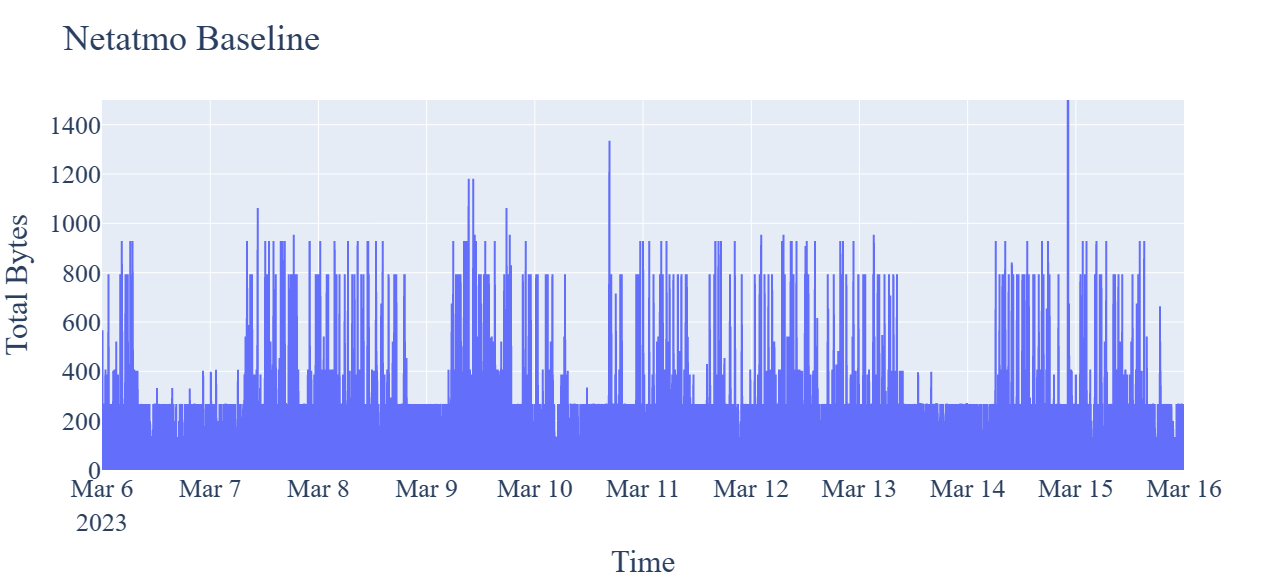
\includegraphics[scale=0.3]{figures/Netatmo_Baseline_TotalBytes.png}
    \caption{Netatmo Baseline Total Bytes}
    \label{fig:NetatmoBaselineTotalBytes}
\end{figure}

\begin{figure} [H]         
    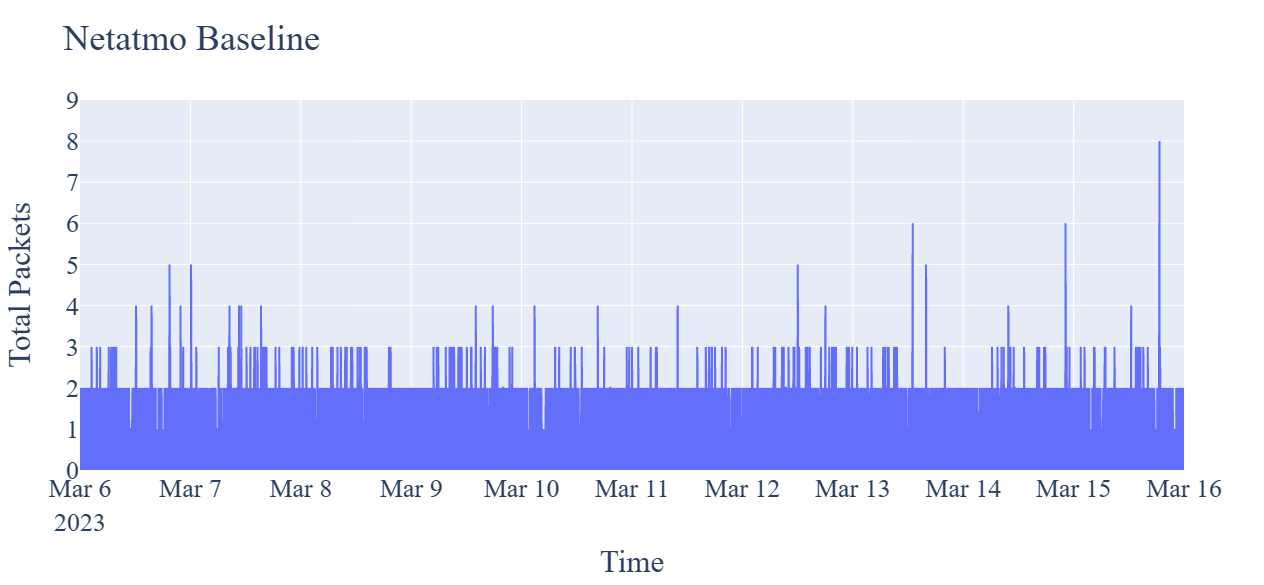
\includegraphics[scale=0.3]{figures/Netatmo_Baseline_TotalPackets.png}
    \caption{Netatmo Baseline Total Packets}
    \label{fig:NetatmoBaselineTotalPackets}
 \end{figure}

For the baseline graphs, it is possible to see that packets are sent continually at a rate of around 250 bytes per 2 seconds and 2 packets per 2 seconds. As these graphs shows the total packets and bytes sent and received, it can also be beneficial to look at what the graphs would look like if filtered on packets and bytes sent and packets and bytes received separately. 

\begin{figure}[H]
    \centering
    \begin{subfigure}[b]{0.7\textwidth}
        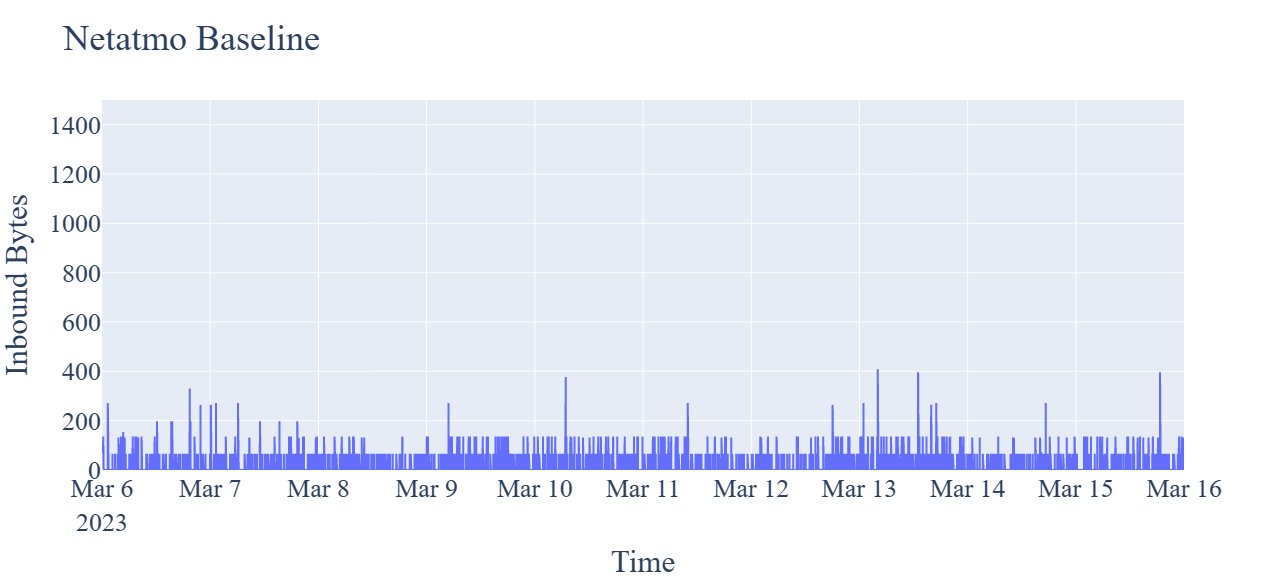
\includegraphics[width=\textwidth]{figures/Netatmo_Baseline_InboundBytes.png}
        \caption{Inbound Bytes}
        \label{fig:NetatmoBaselineInboundBytes}
    \end{subfigure}
    \begin{subfigure}[b]{0.7\textwidth}
        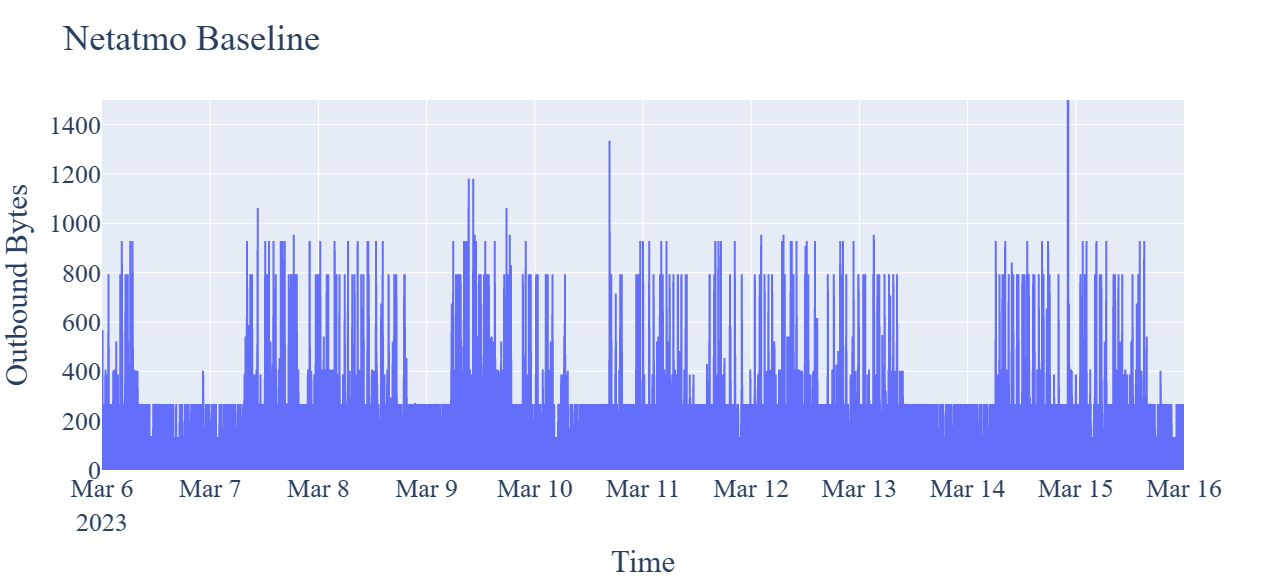
\includegraphics[width=\textwidth]{figures/Netatmo_Baseline_OutboundBytes.png}
        \caption{Outbound Bytes}
        \label{fig:NetatmoBaselineOutboundBytes}
    \end{subfigure}
    \caption{Netatmo Baseline Inbound and Outbound Bytes}
    \label{Fig:NetatmoBaselineOutandInboundBytes}
 \end{figure}

 \begin{figure}[H]
    \centering
    \begin{subfigure}[b]{0.7\textwidth}
        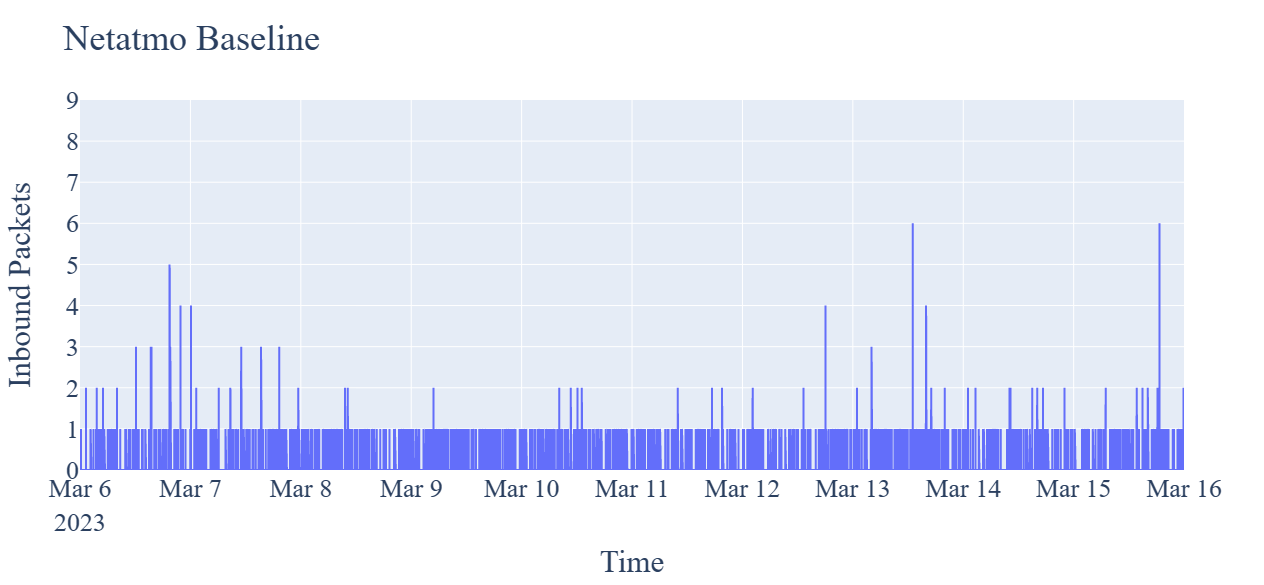
\includegraphics[width=\textwidth]{figures/Netatmo_Baseline_InboundPackets.png}
        \caption{Inbound Packets}
        \label{fig:NetatmoBaselineInboundPackets}
    \end{subfigure}
    \begin{subfigure}[b]{0.7\textwidth}
        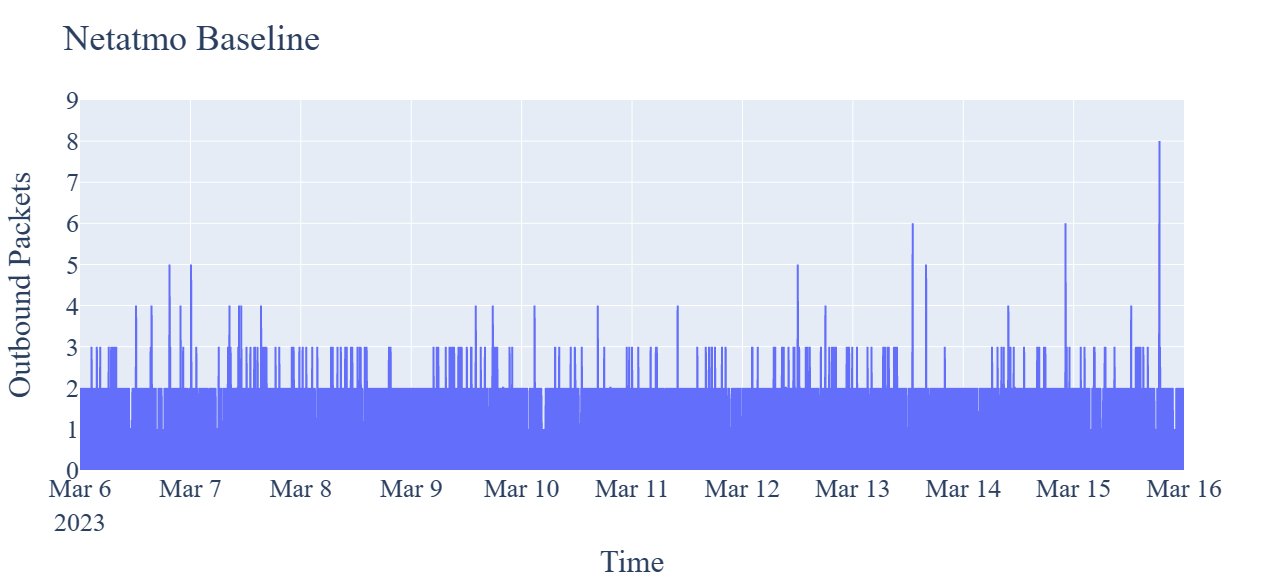
\includegraphics[width=\textwidth]{figures/Netatmo_Baseline_OutboundPackets.png}
        \caption{Outbound Packets}
        \label{fig:NetatmoBaselineOutboundPackets}
    \end{subfigure}
    \caption{Netatmo Baseline Inbound and Outbound Packets}
    \label{Fig:NetatmoBaselineOutandInboundPackets}
 \end{figure}
For the inbound and outbound bytes for Netatmo, \textit{figure \ref{Fig:NetatmoBaselineOutandInboundBytes}}, it is clear to see that the device sends a lot more bytes than it receives. The same pattern appears in \textit{figure \ref{Fig:NetatmoBaselineOutandInboundPackets}} for packets. Calculations made on the baseline traffic are presented in table \ref{tab:NetatmoBaselineCalculations}. 
\begin{table}[H]
    \caption{Calculations for Netatmo Baseline Capture}
    \centering
    \begin{tabular}{ll|l|}
        \cline{3-3}                                               &                               &             \textbf{Numbers} \\ \hline
        \multicolumn{1}{|c|}{\multirow{4}{*}{\textbf{Total}}}    & Packets              & 110,735         \\ \cline{2-3} 
        \multicolumn{1}{|c|}{}                                   & Bytes                & 14,959,396       \\ \cline{2-3} 
        \multicolumn{1}{|c|}{}                                   & Average bytes/second & 17               \\ \cline{2-3} 
        \multicolumn{1}{|c|}{}                                   & Average packet size  & 135 bytes        \\ \hline
        \multicolumn{1}{|l|}{\multirow{5}{*}{\textbf{Inbound}}}  & Packets              & 1,042            \\ \cline{2-3} 
        \multicolumn{1}{|l|}{}                                   & Bytes                & 83,446           \\ \cline{2-3} 
        \multicolumn{1}{|l|}{}                                   & Average bytes/second & 0                \\ \cline{2-3} 
        \multicolumn{1}{|l|}{}                                   & Average packet size  & 80 bytes          \\ \cline{2-3} 
        \multicolumn{1}{|l|}{}                                   & Biggest packet       & 377 bytes        \\ \hline
        \multicolumn{1}{|l|}{\multirow{5}{*}{\textbf{Outbound}}} & Packets              & 109,693          \\ \cline{2-3} 
        \multicolumn{1}{|l|}{}                                   & Bytes                & 14,875,950       \\ \cline{2-3} 
        \multicolumn{1}{|l|}{}                                   & Average bytes/second & 17               \\ \cline{2-3} 
        \multicolumn{1}{|l|}{}                                   & Average packet size  & 136 bytes         \\ \cline{2-3} 
        \multicolumn{1}{|l|}{}                                   & Biggest packet       & 1,150 bytes       \\ \hline
    \end{tabular}
    \label{tab:NetatmoBaselineCalculations}
\end{table}
Comparing the inbound(figure \ref{fig:NetatmoBaselineInboundBytes} and \ref{fig:NetatmoBaselineInboundPackets}) and outbound(figure \ref{fig:NetatmoBaselineOutboundBytes} and \ref{fig:NetatmoBaselineOutboundPackets}) graphs with the total graphs (figure \ref{fig:NetatmoBaselineTotalBytes} and figures \ref{fig:NetatmoBaselineTotalPackets}), shows that the outbound graphs stands for a majority of the packets and they are very similar to the total graphs. The same is numerically shown in table \ref{tab:NetatmoBaselineCalculations}, where over 99\% of the total packets are outbound traffic. The majority of packets sent from Netatmo are packets labeled "Data" with a size of 134 bytes, which makes up 98,3\% of the packets from the capture file. Therefore, it will be better to only display the events with graphs for total traffic to evaluate and analyze further on. 

\subsection{Mill Baseline}
\textit{Figure \ref{fig:MillBaselineTotalPackets}} and \textit{\ref{fig:MillBaselineTotalBytes}} shows the graphs for Mill from the baseline capturing from 6th of March 2023 to 15th of March 2023. 
\begin{figure} [H]
    \centering
    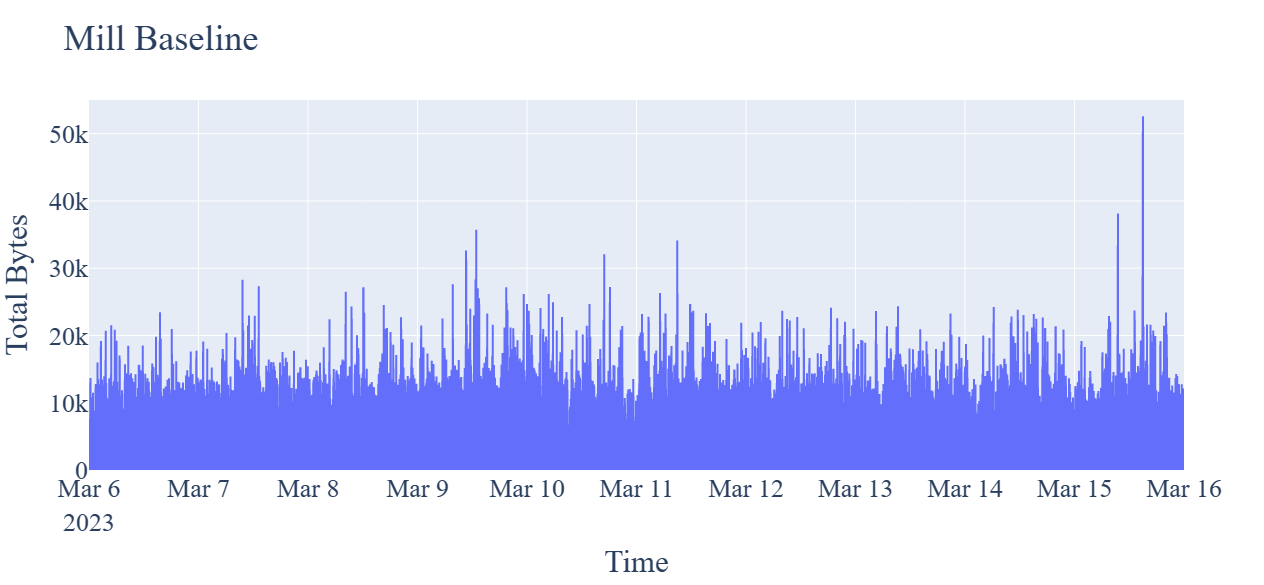
\includegraphics[scale=0.3]{figures/Mill_Baseline_TotalBytes.png}
    \caption{Mill Baseline Total Bytes}
    \label{fig:MillBaselineTotalBytes}
\end{figure}

\begin{figure} [H]
    \centering
    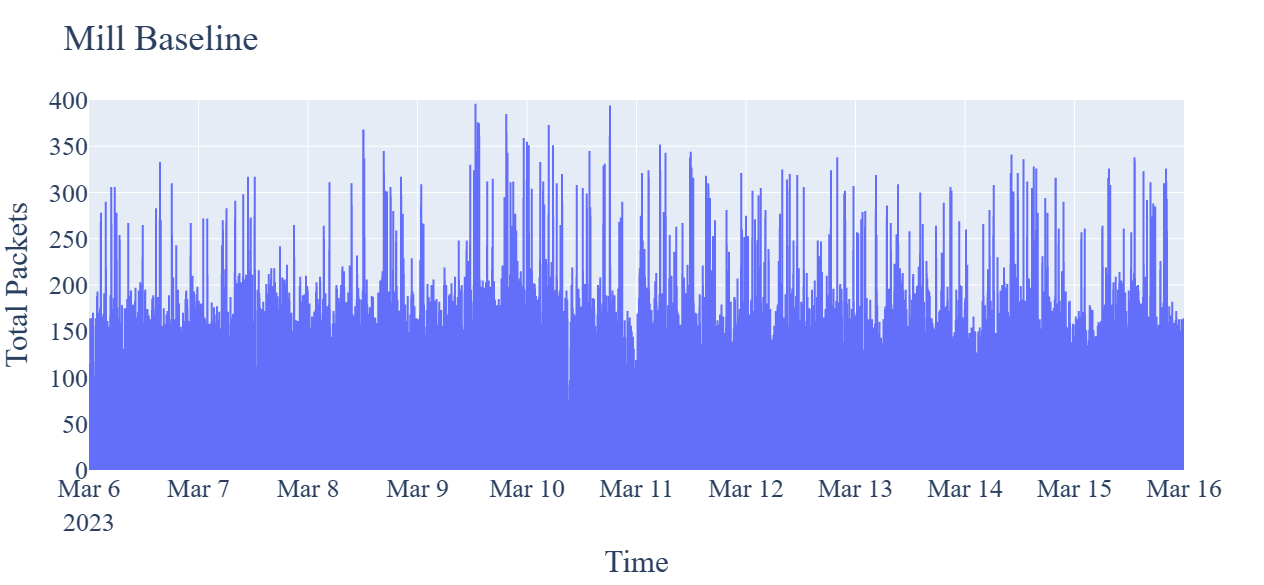
\includegraphics[scale=0.3]{figures/Mill_Baseline_TotalPackets.png}
    \caption{Mill Baseline Total Packets}
    \label{fig:MillBaselineTotalPackets}
 \end{figure}

The baseline traffic for Mill shows that the traffic varies a lot. As this device does not send live updates, but every minute, more spikes are included as it does not always send packets. It is also possible to see the spikes more clearly if the time range is smaller, this will be visible further when looking at the baseline comparison graphs for each event. 

Graphs for inbound and outbound traffic have also been made for Mill, to see the differences for the packets sent. Figure \ref{Fig:MillBaselineOutandInboundBytes} and \ref{Fig:MillBaselineOutandInboundPackets} displays the different graphs for each of the traffic directions. Numerical calculations for the baseline traffic are presented in table \ref{tab:MillBaselineCalculations}. 

\begin{figure}[H]
    \centering
    \begin{subfigure}[b]{0.7\textwidth}
        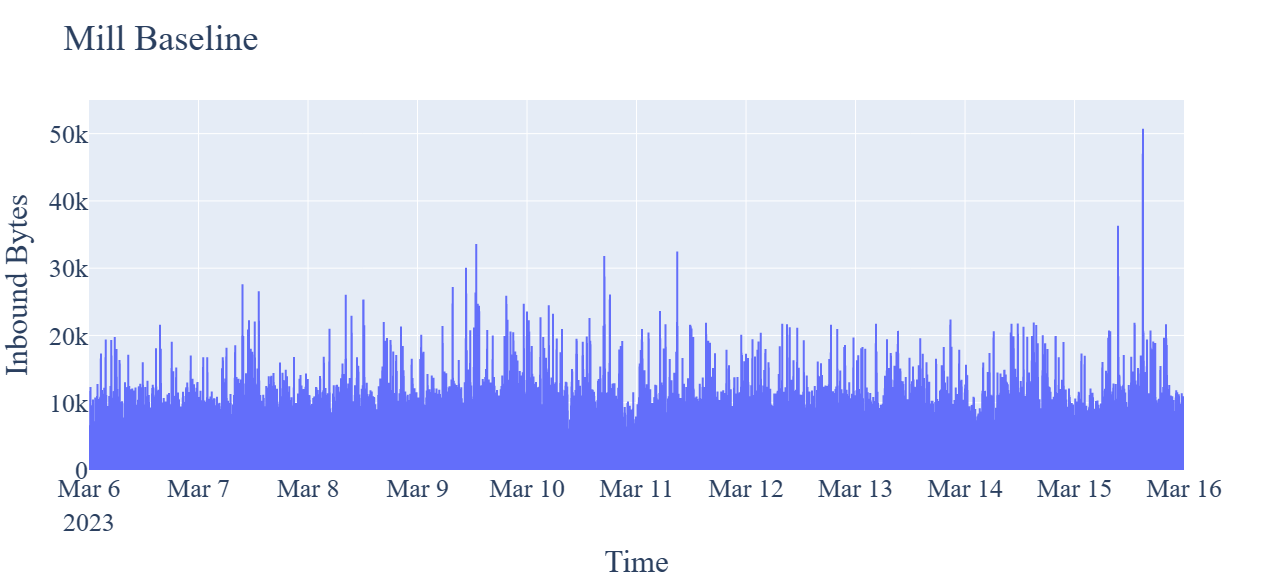
\includegraphics[width=\textwidth]{figures/Mill_Baseline_InboundBytes.png}
        \caption{Inbound Bytes}
        \label{fig:MillBaselineInboundBytes}
    \end{subfigure}
    \begin{subfigure}[b]{0.7\textwidth}
        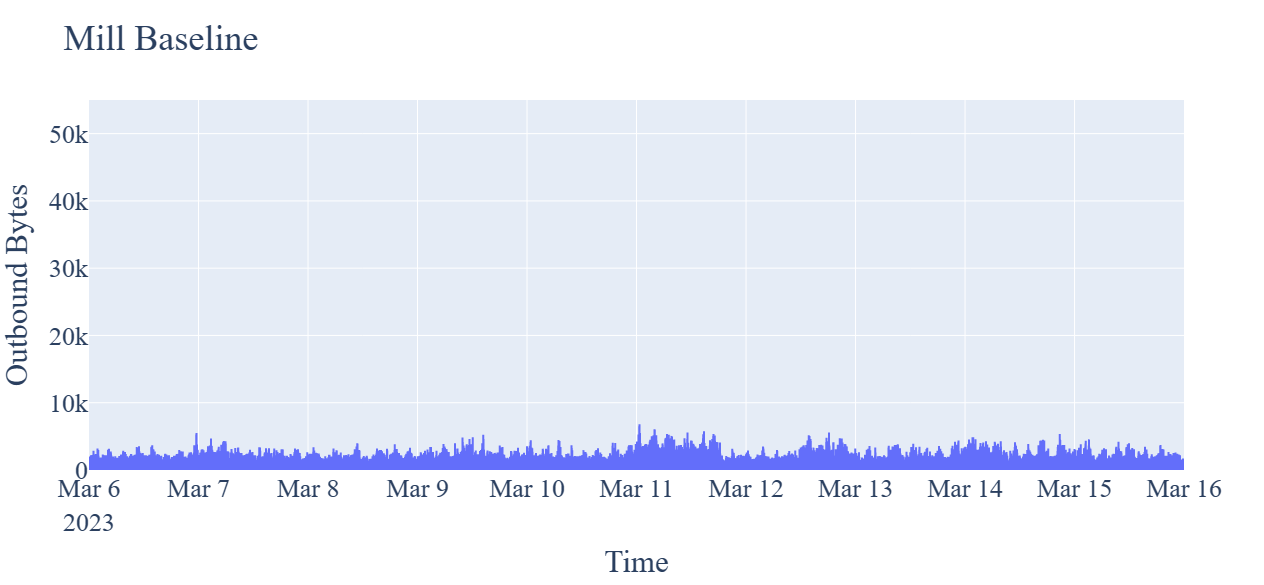
\includegraphics[width=\textwidth]{figures/Mill_Baseline_OutboundBytes.png}
        \caption{Outbound Bytes}
        \label{fig:MillBaselineOutboundBytes}
    \end{subfigure}
    \caption{Mill Baseline Inbound and Outbound Bytes}
    \label{Fig:MillBaselineOutandInboundBytes}
 \end{figure}

 \begin{figure}[H]
    \centering
    \begin{subfigure}[b]{0.7\textwidth}
        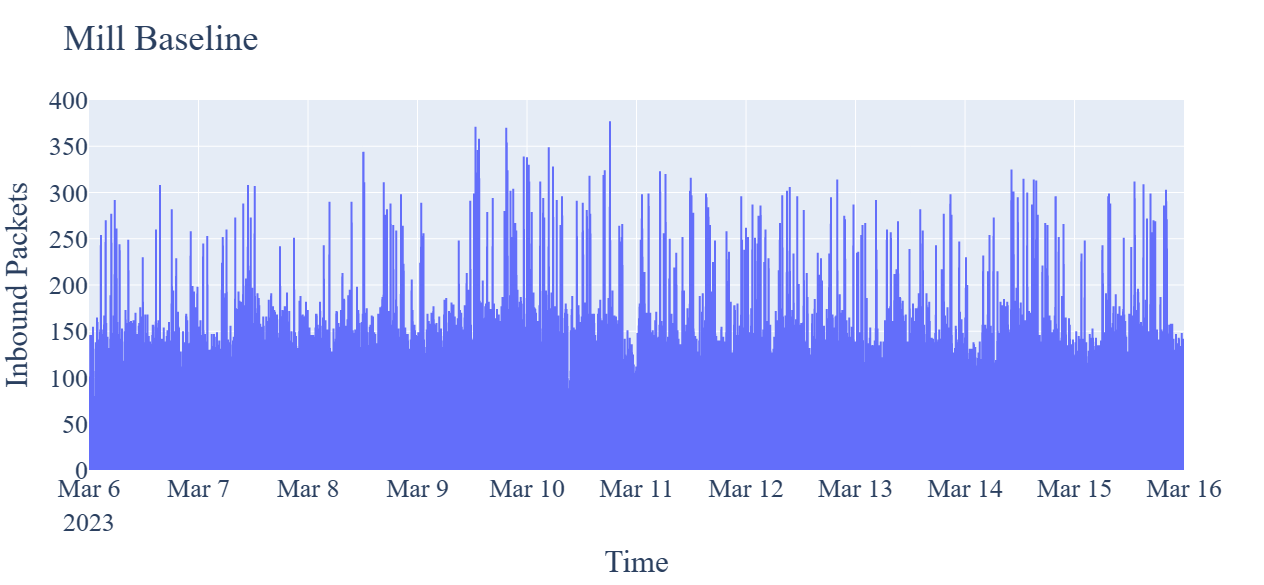
\includegraphics[width=\textwidth]{figures/Mill_Baseline_InboundPackets.png}
        \caption{Inbound Packets}
        \label{fig:MillBaselineInboundPackets}
    \end{subfigure}
    \begin{subfigure}[b]{0.7\textwidth}
        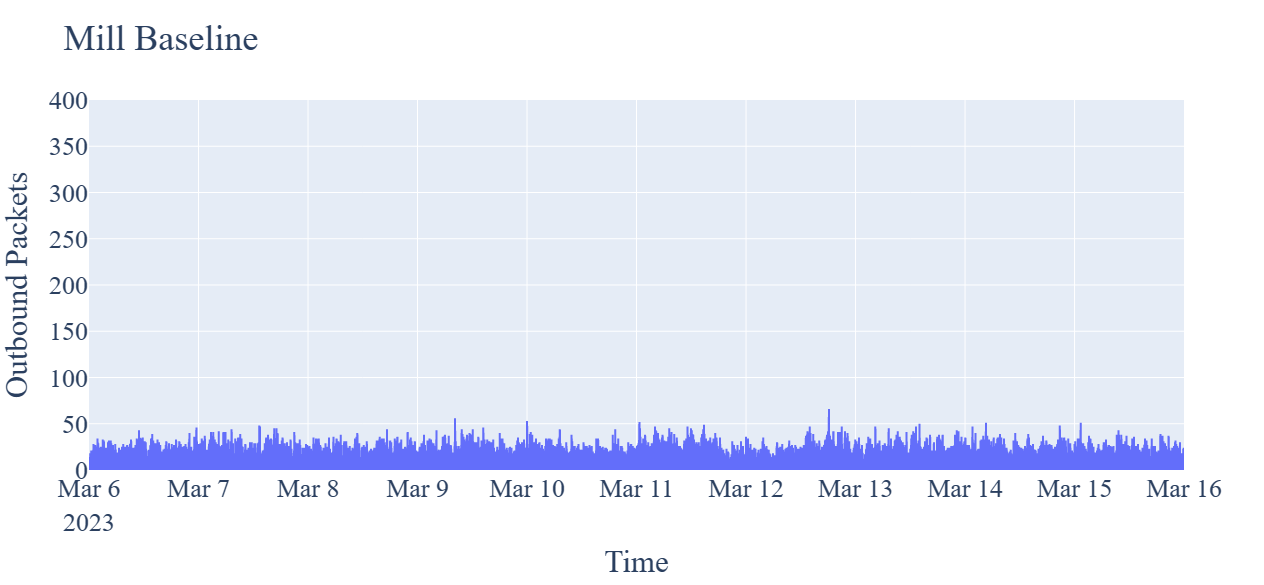
\includegraphics[width=\textwidth]{figures/Mill_Baseline_OutboundPackets.png}
        \caption{Outbound Packets}
        \label{fig:MillBaselineOutboundPackets}
    \end{subfigure}
    \caption{Mill Baseline Inbound and Outbound Packets}
    \label{Fig:MillBaselineOutandInboundPackets}
 \end{figure}

\begin{table}[H]
    \caption{Calculations for Mill Baseline Capture}
    \centering
    \begin{tabular}{ll|l|}
        \cline{3-3}                                              &                      & \textbf{Numbers} \\ \hline
        \multicolumn{1}{|c|}{\multirow{4}{*}{\textbf{Total}}}    & Packets              & 1,236,753       \\ \cline{2-3} 
        \multicolumn{1}{|c|}{}                                   & Bytes                & 129,253,290     \\ \cline{2-3} 
        \multicolumn{1}{|c|}{}                                   & Average bytes/second & 149             \\ \cline{2-3} 
        \multicolumn{1}{|c|}{}                                   & Average packet size  & 105 bytes       \\ \hline
        \multicolumn{1}{|l|}{\multirow{5}{*}{\textbf{Inbound}}}  & Packets              & 942,112         \\ \cline{2-3} 
        \multicolumn{1}{|l|}{}                                   & Bytes                & 95,458,773      \\ \cline{2-3} 
        \multicolumn{1}{|l|}{}                                   & Average bytes/second & 110             \\ \cline{2-3} 
        \multicolumn{1}{|l|}{}                                   & Average packet size  & 101 bytes       \\ \cline{2-3} 
        \multicolumn{1}{|l|}{}                                   & Biggest packet       & 1593 bytes      \\ \hline
        \multicolumn{1}{|l|}{\multirow{5}{*}{\textbf{Outbound}}} & Packets              & 294,640         \\ \cline{2-3} 
        \multicolumn{1}{|l|}{}                                   & Bytes                & 33,794,517      \\ \cline{2-3} 
        \multicolumn{1}{|l|}{}                                   & Average bytes/second & 39              \\ \cline{2-3} 
        \multicolumn{1}{|l|}{}                                   & Average packet size  & 115 bytes       \\ \cline{2-3} 
        \multicolumn{1}{|l|}{}                                   & Biggest packet       & 456 bytes       \\ \hline
    \end{tabular}
    \label{tab:MillBaselineCalculations}
\end{table}

As figure \ref{Fig:MillBaselineOutandInboundBytes} and \ref{Fig:MillBaselineOutandInboundPackets} shows, the device receives a lot more packets and bytes than it sends off. And as the inbound graphs do not differ much from the total graphs, it will be best to proceed with the analysis in a total traffic aspect where both inbound and outbound traffic are included. This is also reflected in table \ref{tab:MillBaselineCalculations}, which shows that 76\% of packets and 74\% of bytes are received.

\subsection{Nedis Baseline}
\textit{Figure \ref{fig:NedisBaselineTotalPackets}} and \textit{\ref{fig:NedisBaselineTotalBytes}} shows the graphs for Nedis from the baseline capturing from 6th of March 2023 to 15th of March 2023. 
\begin{figure} [H]
    \centering
    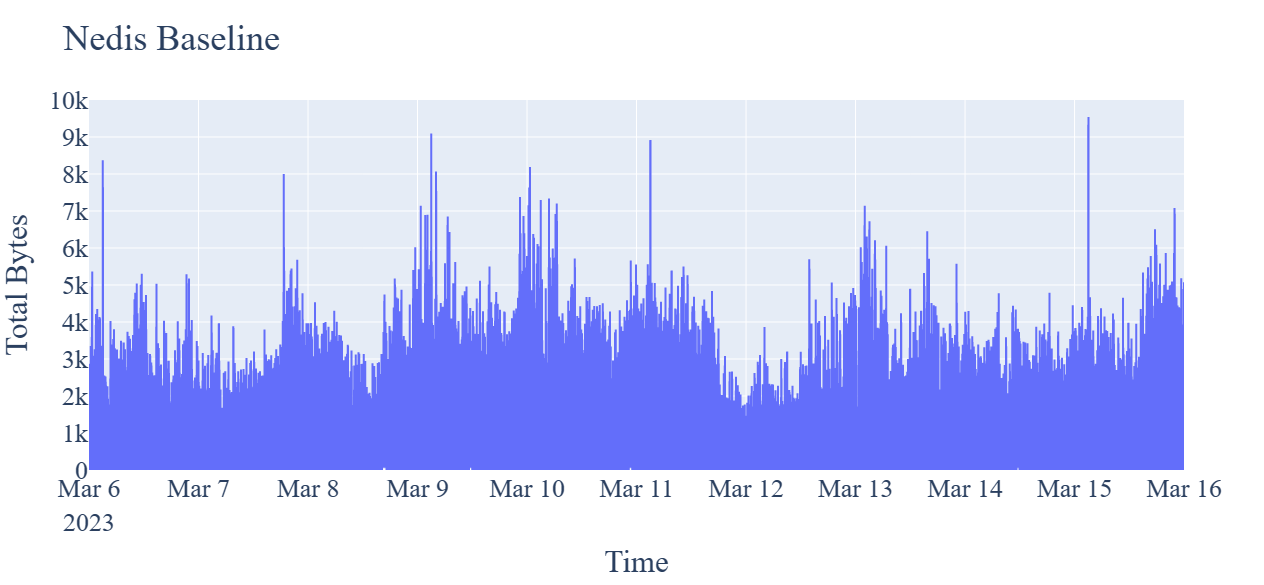
\includegraphics[scale=0.3]{figures/Nedis_Baseline_TotalBytes.png}
    \caption{Nedis Baseline Total Bytes}
    \label{fig:NedisBaselineTotalBytes}
\end{figure}

\begin{figure} [H]         
    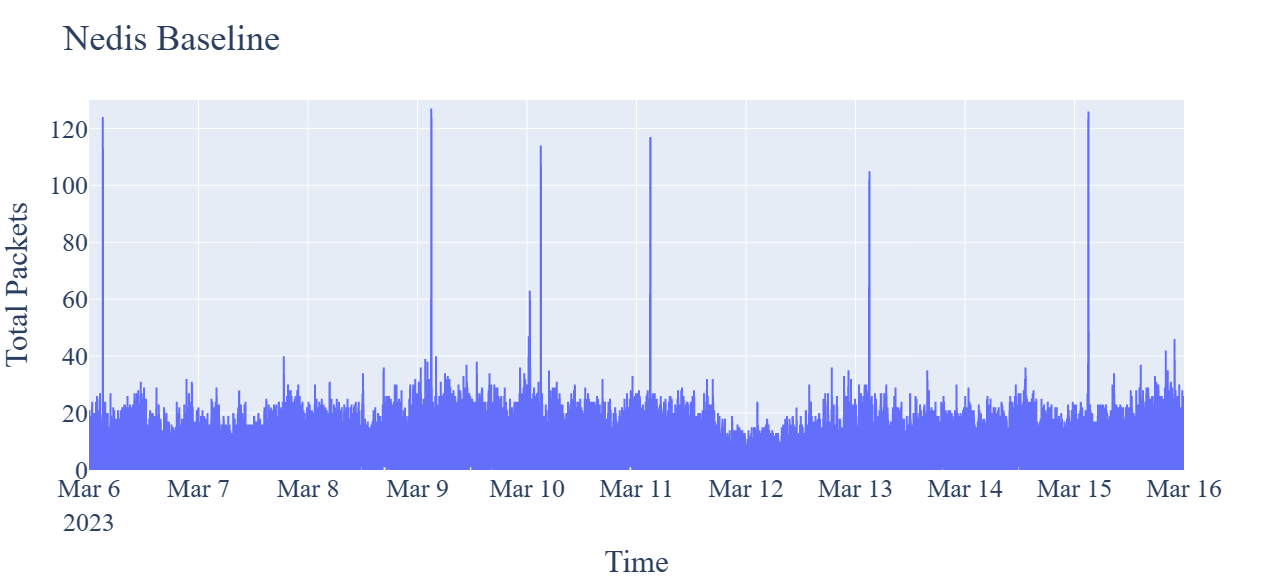
\includegraphics[scale=0.3]{figures/Nedis_Baseline_TotalPackets.png}
    \caption{Nedis Baseline Total Packets}
    \label{fig:NedisBaselineTotalPackets}
 \end{figure}

The traffic sent and received by Nedis is characterized by several spikes even though the traffic varies some. The larger spikes, which are more visible in figure \ref{fig:NedisBaselineTotalPackets}, showing the packets, occurs almost everyday. Since traffic is encrypted, it is not possible to see what these spikes are, but for further analysis it is important to understand that normal traffic for the device, can be large spikes occurring around the same time each night the spike occurs. Even though this thesis will not go further into looking at what the spikes actually are, it can be interesting to see if they are inbound or outbound traffic. 

To look at the differences in inbound and outbound traffic for Nedis, figure \ref{Fig:NedisBaselineOutandInboundBytes} and \ref{Fig:NedisBaselineOutandInboundPackets} are displayed. Figure \ref{fig:NedisBaselineOutboundPackets} shows that the spikes are packets which the device receives.
Even though the graphs for inbound and outbound traffic from Nedis looks more similar, the calculations presented in table \ref{tab:NedisBaselineCalculations}, shows that 81\% of the packets and 70\% of the bytes in the baseline are traffic sent from the device. Looking at the graphs in total will therefore give the most to analyze. Another aspect of looking at the graphs in total, compared to inbound and outbound separately is that since the traffic is encrypted on the layer 2, it is not possible to know what makes the possible changes. 

\begin{figure}[H]
    \centering
    \begin{subfigure}[b]{0.7\textwidth}
        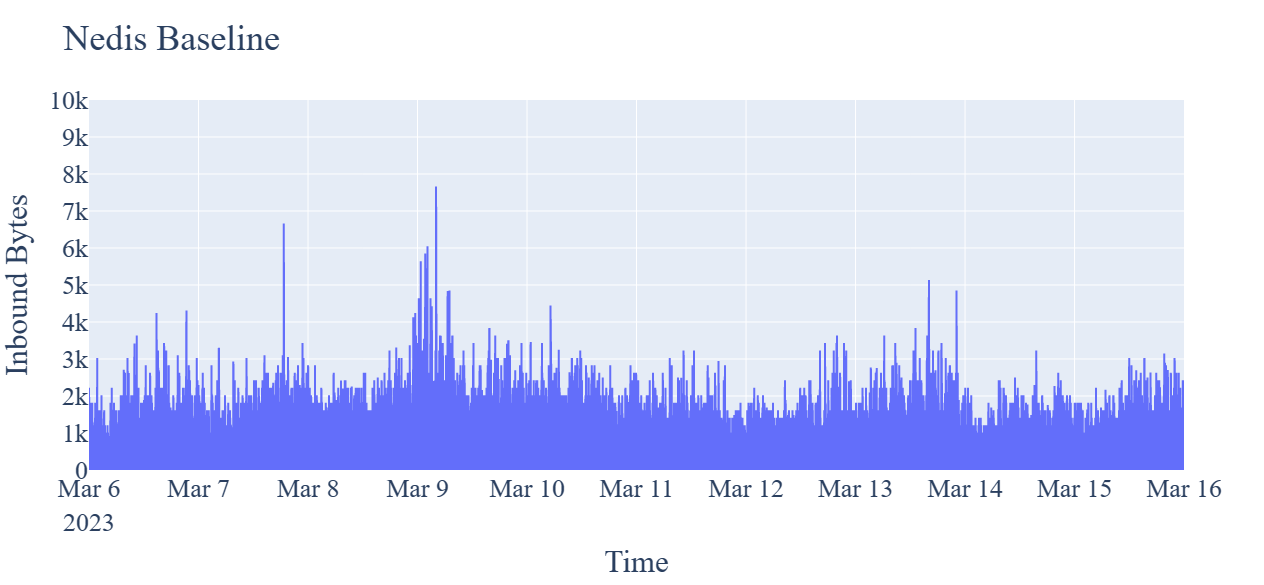
\includegraphics[width=\textwidth]{figures/Nedis_Baseline_InboundBytes.png}
        \caption{Inbound Bytes}
        \label{fig:NedisBaselineInboundBytes}
    \end{subfigure}
    \begin{subfigure}[b]{0.7\textwidth}
        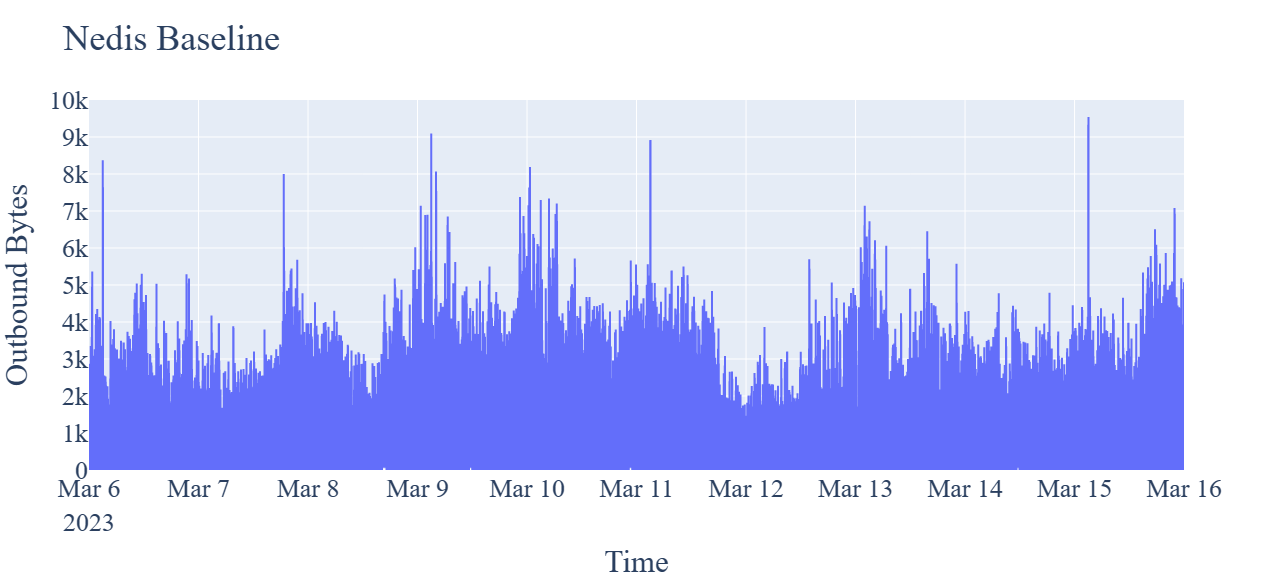
\includegraphics[width=\textwidth]{figures/Nedis_Baseline_OutboundBytes.png}
        \caption{Outbound Bytes}
        \label{fig:NedisBaselineOutboundBytes}
    \end{subfigure}
    \caption{Nedis Baseline Inbound and Outbound Bytes}
    \label{Fig:NedisBaselineOutandInboundBytes}
 \end{figure}

 \begin{figure}[H]
    \centering
    \begin{subfigure}[b]{0.7\textwidth}
        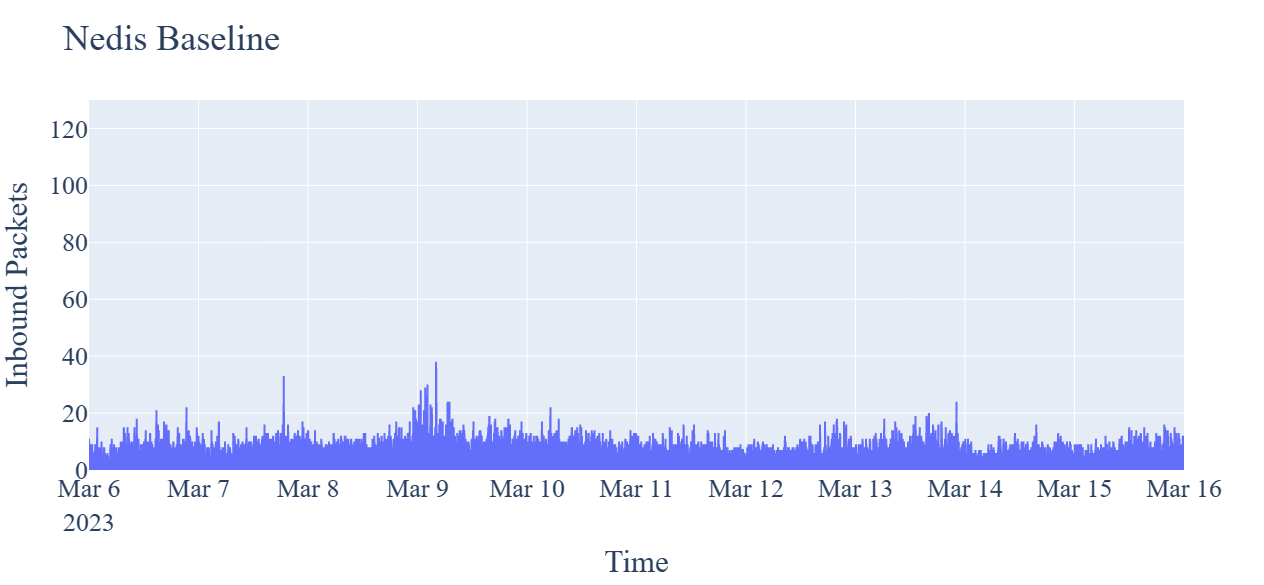
\includegraphics[width=\textwidth]{figures/Nedis_Baseline_InboundPackets.png}
        \caption{Inbound Packets}
        \label{fig:NedisBaselineInboundPackets}
    \end{subfigure}
    \begin{subfigure}[b]{0.7\textwidth}
        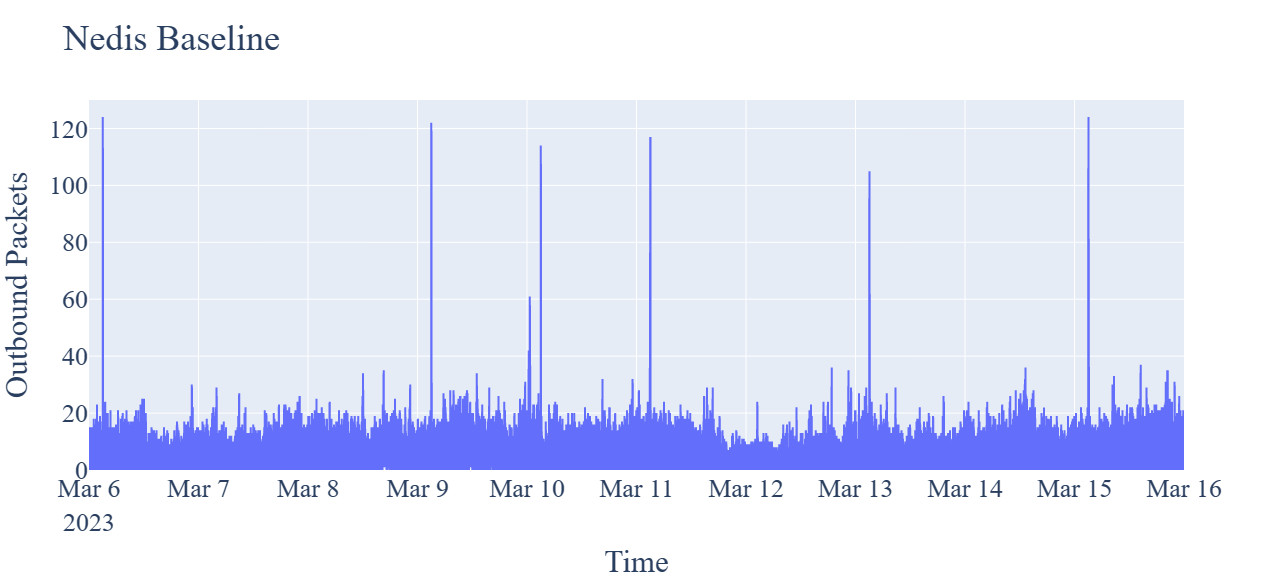
\includegraphics[width=\textwidth]{figures/Nedis_Baseline_OutboundPackets.png}
        \caption{Outbound Packets}
        \label{fig:NedisBaselineOutboundPackets}
    \end{subfigure}
    \caption{Nedis Baseline Inbound and Outbound Packets}
    \label{Fig:NedisBaselineOutandInboundPackets}
 \end{figure}
 
\begin{table}[H]
    \caption{Calculations for Nedis Baseline Capture}
    \centering
    \begin{tabular}{ll|l|}
        \cline{3-3}                                               &                               &             \textbf{Numbers} \\ \hline
        \multicolumn{1}{|c|}{\multirow{4}{*}{\textbf{Total}}}    & Packets              & 2,428,701         \\ \cline{2-3} 
        \multicolumn{1}{|c|}{}                                   & Bytes                & 295,022,494       \\ \cline{2-3} 
        \multicolumn{1}{|c|}{}                                   & Average bytes/second & 341               \\ \cline{2-3} 
        \multicolumn{1}{|c|}{}                                   & Average packet size  & 121 bytes        \\ \hline
        \multicolumn{1}{|l|}{\multirow{5}{*}{\textbf{Inbound}}}  & Packets              & 451,495           \\ \cline{2-3} 
        \multicolumn{1}{|l|}{}                                   & Bytes                & 88,595,049        \\ \cline{2-3} 
        \multicolumn{1}{|l|}{}                                   & Average bytes/second & 102                \\ \cline{2-3} 
        \multicolumn{1}{|l|}{}                                   & Average packet size  & 196 bytes         \\ \cline{2-3} 
        \multicolumn{1}{|l|}{}                                   & Biggest packet       & 522 bytes        \\ \hline
        \multicolumn{1}{|l|}{\multirow{5}{*}{\textbf{Outbound}}} & Packets              & 1,977,206         \\ \cline{2-3} 
        \multicolumn{1}{|l|}{}                                   & Bytes                & 206,427,445      \\ \cline{2-3} 
        \multicolumn{1}{|l|}{}                                   & Average bytes/second & 238               \\ \cline{2-3} 
        \multicolumn{1}{|l|}{}                                   & Average packet size  & 104 bytes         \\ \cline{2-3} 
        \multicolumn{1}{|l|}{}                                   & Biggest packet       & 485 bytes       \\ \hline
    \end{tabular}
    \label{tab:NedisBaselineCalculations}
\end{table} 


\section{Test Case 1: Cooking}
This chapter presents the results and analysis conducted on Test Case 1: Cooking. The first subsection will present general information applicable to all the devices, and the following subsections will present the result and analysis for each of the devices separately. 
\subsection{General}
The cooking events are 15 in total and are presented in table \ref{tab:CookingDates}. Every device has the same dates for this event. 
\begin{table}[!hbtp]
    \centering
    \caption{Date and time for Test Case 1: Cooking Events}
    \begin{adjustbox}{width=1\textwidth}
            \begin{tabular}{l|l|l|l|l|l|l|l|l|l|l|l|l|l|l|l|}
            \cline{2-16} 
            & 08.01 & 09.01 & 10.01 & 11.01 & 12.01 & 16.01 & 18.01 & 19.01 & 24.01 & 25.01 & 26.01 & 30.01 & 31.01 & 01.02 & 02.02 \\
            \hline
            \multicolumn{1}{|l|}{Started event}  & 15:58 & 15:59 & 16:01 & 16:05 & 16:10 & 16:02 & 16:04 & 16:01 & 15:57 & 16:02 & 16:01 & 16:01 & 16:01 & 16:02 & 16:02 \\ 
            \hline
            \multicolumn{1}{|l|}{Finished event} & 16:22 & 16:21 & 16:27 & 16:37 & 16:28 & 16:25 & 16:25 & 16:18 & 16:20 & 16:13 & 16:25 & 16:19 & 16:21 & 16:22 & 16:22 \\ 
            \hline
            \end{tabular}
    \end{adjustbox}
    \label{tab:CookingDates}
\end{table}
\FloatBarrier

To be able to look even further into differences from when the devices are in an environment when an event is ongoing and when it is in the same environment, but without any event ongoing, graphs and calculations from the baseline traffic are used to compare. To choose a time for the baseline traffic, all start values from the actual events in table \ref{tab:CookingDates} are used to calculate an average value for starting time. The same applies to end time. Calculated average value for the cooking event is:

\begin{itemize}
    \item Event Start: 15:58
    \item Event Finished: 16:22
\end{itemize}
\newpage

\subsection{Netatmo Home Coach}
The graphs in figure \ref{fig:NetatmoCookingBytes} and \ref{fig:NetatmoCookingPackets} shows both bytes and packets for the first 10 of the cooking events. The area marked red on the graphs are when the event was ongoing. Table \ref{tab:NetatmoCookingCalculations} presents the calculations from all the 15 cooking events. The table also includes average and standard deviation (std deviation) values for the events. 

\begin{table}[!ht]
    \centering
    \caption{Netatmo Cooking Calculations}
    \begin{tabular}{|l|l|l|l|l|l|}
    \hline
        \textbf{Event dates} & \textbf{Packets} & \textbf{Bytes} & \textbf{Biggest packet} & \textbf{Average bytes/s} & \textbf{Average packet size}  \\ \hline
        08.jan & 789 & 107,094 & 407 & 21 & 136 bytes \\ \hline
        09.jan & 589 & 81,694 & 407 & 16 & 139 bytes \\ \hline
        10.jan & 786 & 105,351 & 203 & 20 & 134 bytes \\ \hline
        11.jan & 791 & 107,011 & 407 & 19 & 135 bytes \\ \hline
        12.jan & 528 & 71,873 & 407 & 15 & 136  bytes\\ \hline
        16.jan & 921 & 123,899 & 407 & 24 & 135 bytes \\ \hline
        18.jan & 739 & 108,857 & 407 & 22 & 137 bytes  \\ \hline
        19.jan & 607 & 82,423 & 407 & 17 & 136 bytes \\ \hline
        24.jan & 836 & 114,340 & 407 & 22 & 137 bytes  \\ \hline
        25.jan & 309 & 42,332 & 407 & 10 & 137 bytes \\ \hline
        26.jan & 739 & 100,223 & 407 & 19 & 136 bytes  \\ \hline
        30.jan & 654 & 89,264 & 407 & 19 & 136 bytes \\ \hline
        31.jan & 704 & 93,998 & 136 & 19 & 134 bytes \\ \hline
        01.feb & 644 & 87,474 & 407 & 18 & 136 bytes \\ \hline
        02.feb & 666 & 91,485 & 407 & 19 & 137 bytes \\ \hline
        \textbf{Average} &  \textbf{687}  &  \textbf{93,821}  &  \textbf{375}  &  \textbf{19}  &  \textbf{136 bytes} \\ \hline
        \textbf{Std deviation} &  \textbf{147}  & \textbf{19,914}  &  \textbf{85}  &  \textbf{3}  &  \textbf{1 byte} \\ \hline
    \end{tabular}
    \label{tab:NetatmoCookingCalculations}
\end{table}

\begin{figure}[H]
    \centering
    \begin{subfigure}{0.49\textwidth}
       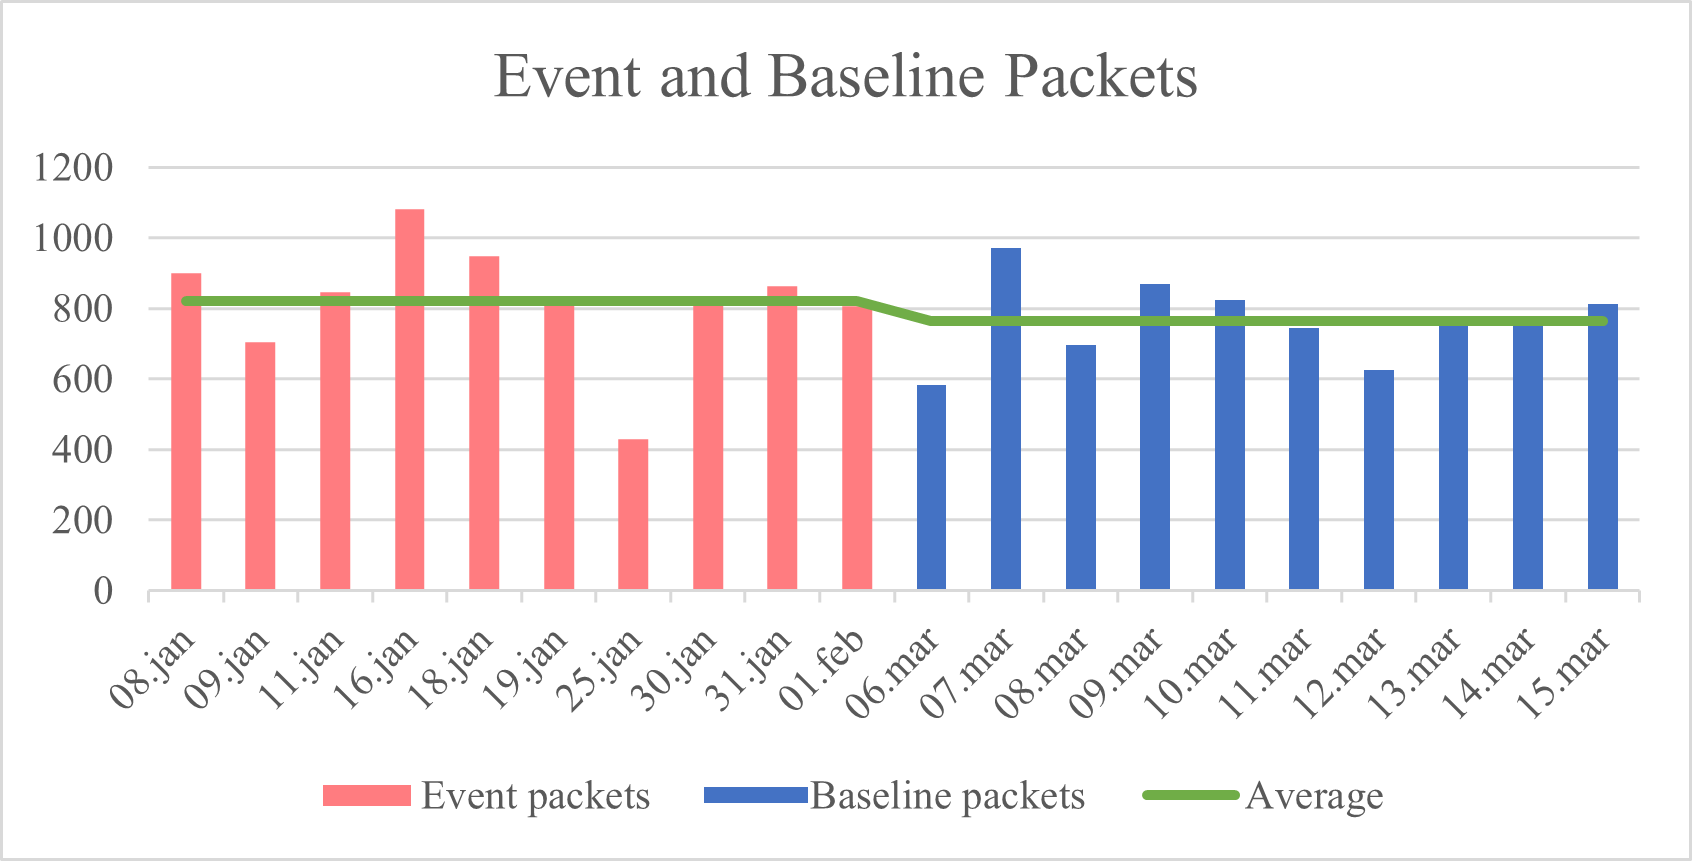
\includegraphics[width=1\hsize]{figures/Netatmo_Cooking_Calculations_Packets.png} 
    \end{subfigure}
    \begin{subfigure}{0.49\textwidth}
        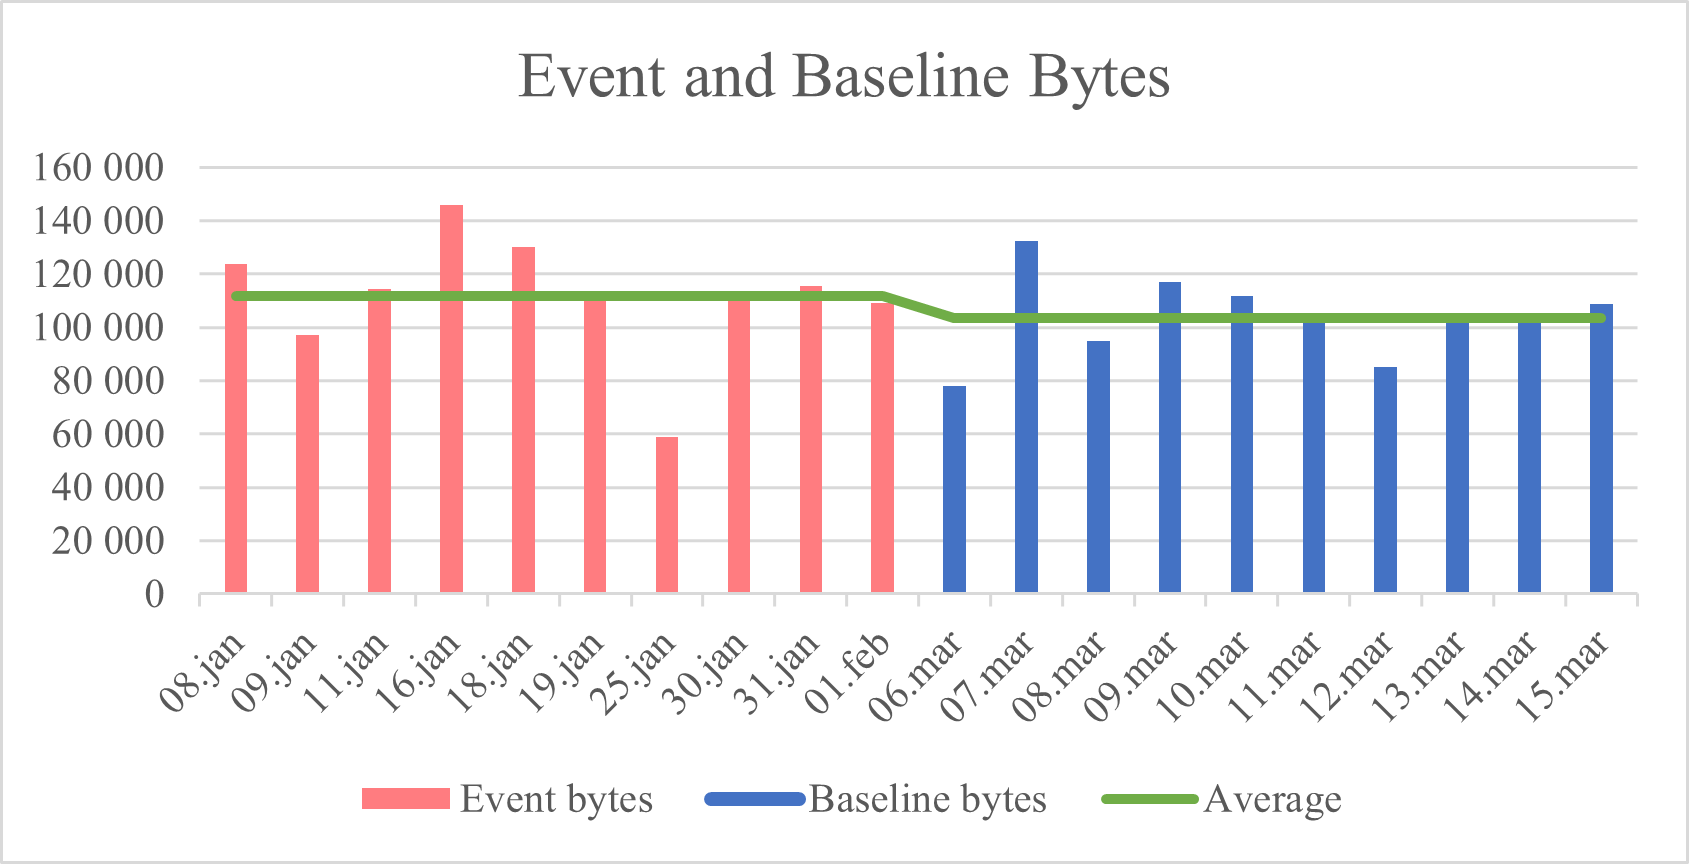
\includegraphics[width=1\hsize]{figures/Netatmo_Cooking_Calculations_Bytes.png} 
    \end{subfigure}
    \caption{Netatmo Cooking Calculations with Packets and Bytes}
    \label{fig:NetatmoCookingCalculations}
\end{figure}

\begin{figure}[H]
    \begin{subfigure}[b]{0.5\textwidth}
        \centering
        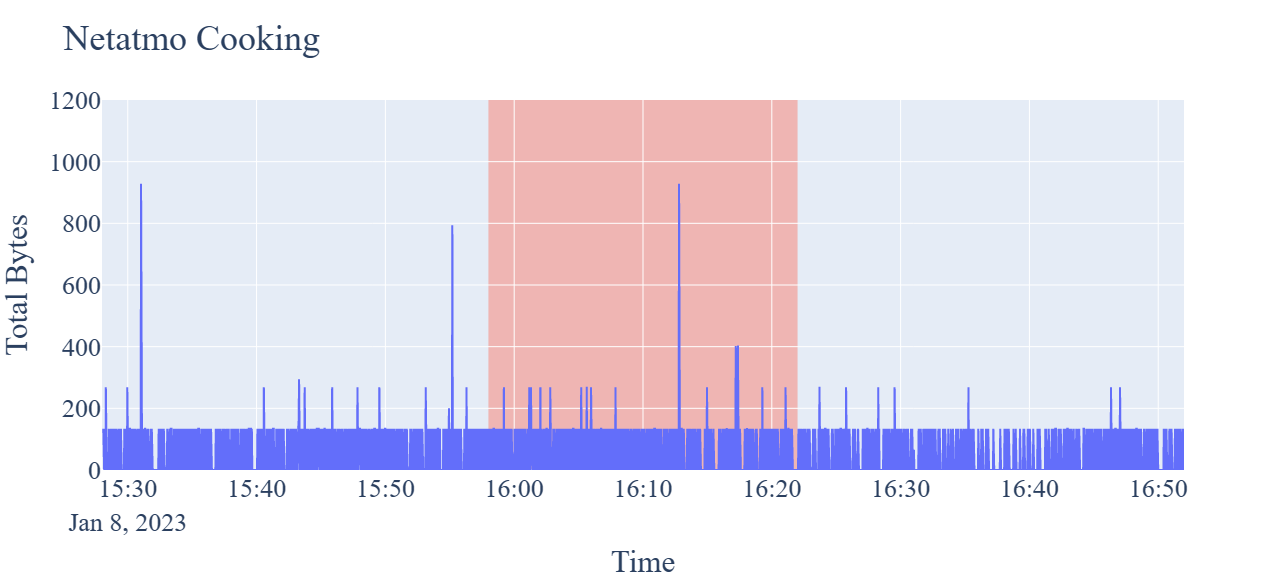
\includegraphics[width=1.2\hsize]{figures/Netatmo_Cooking_Bytes_08.01.png}
    \end{subfigure}
    \begin{subfigure}[b]{0.5\textwidth}
        \centering
        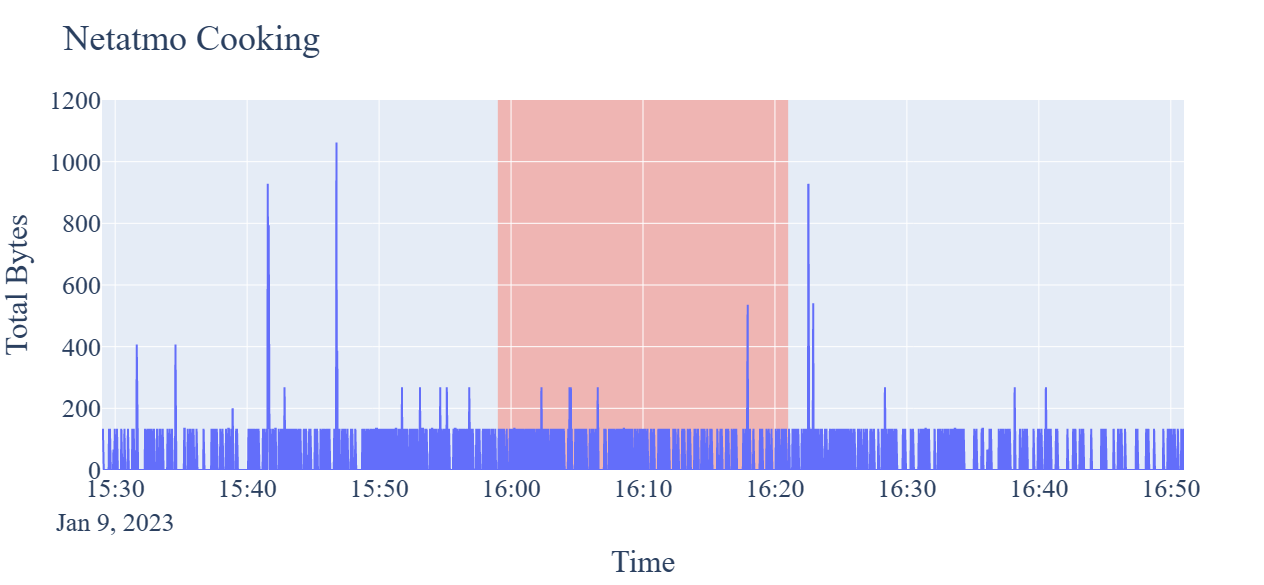
\includegraphics[width=1.2\hsize]{figures/Netatmo_Cooking_Bytes_09.01.png}
    \end{subfigure}
    \begin{subfigure}[b]{0.5\textwidth}
        \centering
        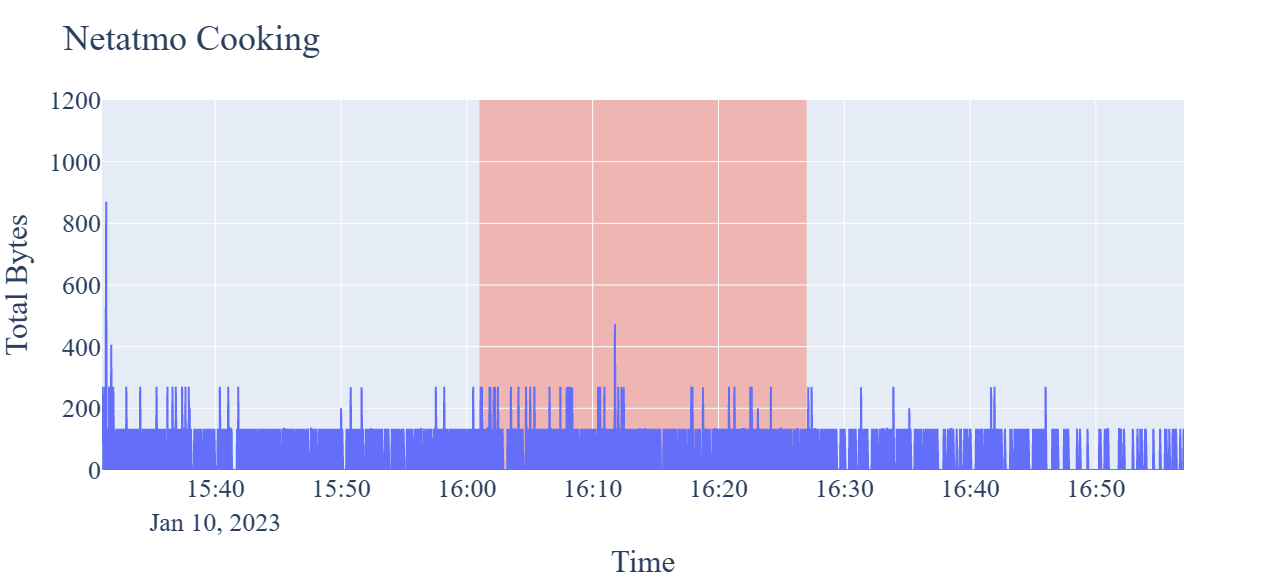
\includegraphics[width=1.2\hsize]{figures/Netatmo_Cooking_Bytes_10.01.png}
    \end{subfigure}
    \begin{subfigure}[b]{0.5\textwidth}
        \centering
        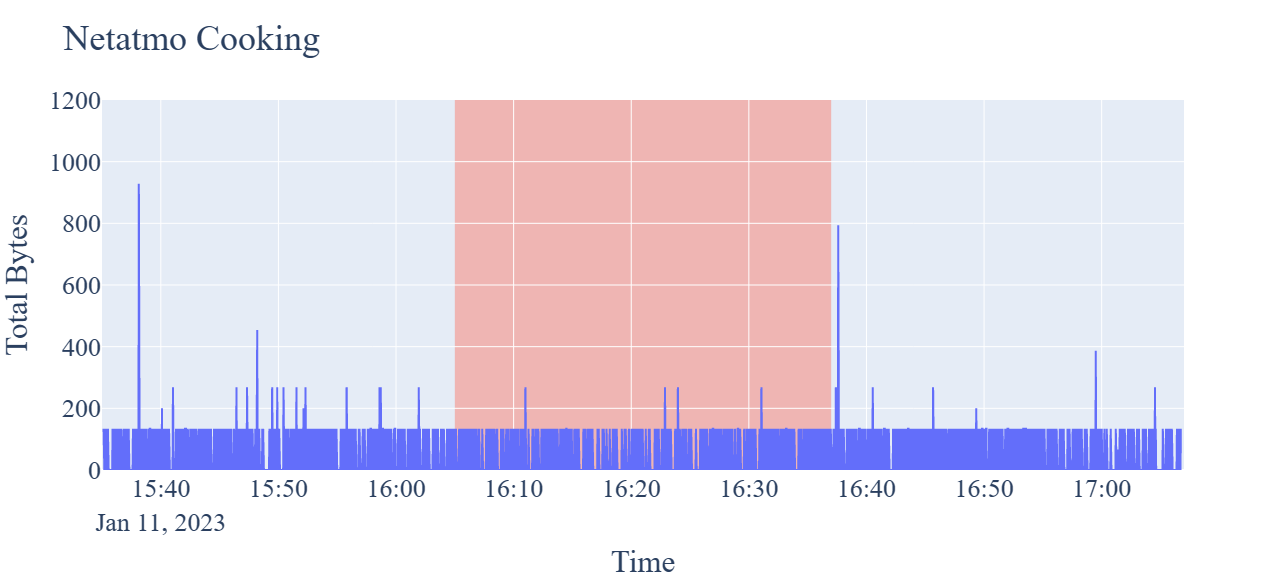
\includegraphics[width=1.2\hsize]{figures/Netatmo_Cooking_Bytes_11.01.png}
    \end{subfigure}
    \begin{subfigure}[b]{0.5\textwidth}
        \centering
        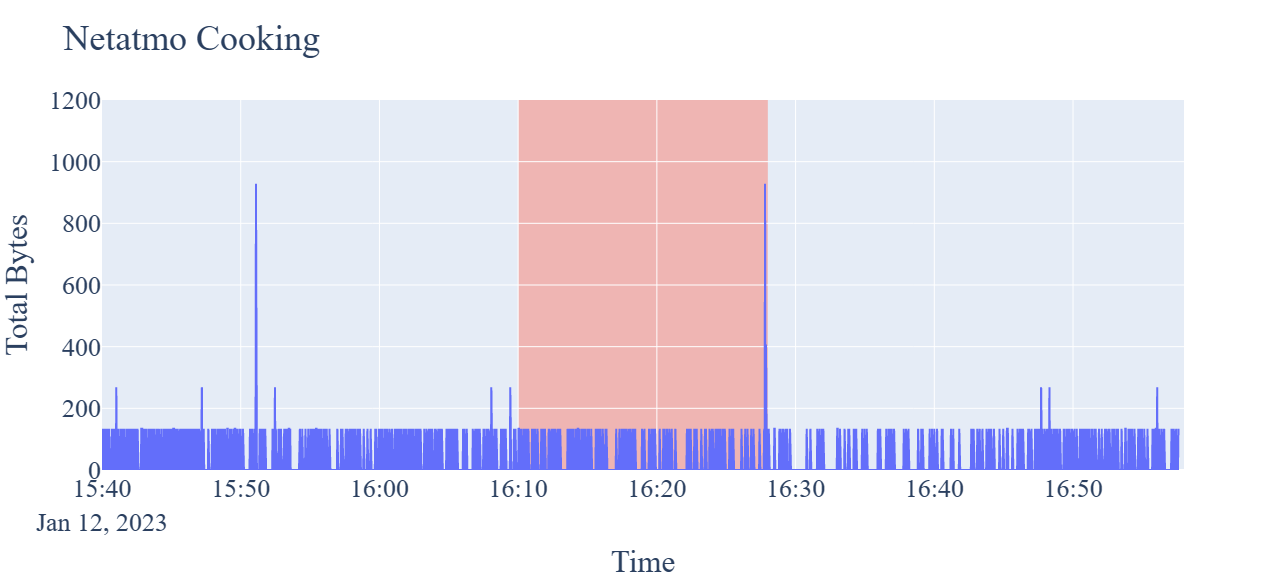
\includegraphics[width=1.2\hsize]{figures/Netatmo_Cooking_Bytes_12.01.png}
    \end{subfigure}
    \begin{subfigure}[b]{0.5\textwidth}
        \centering
        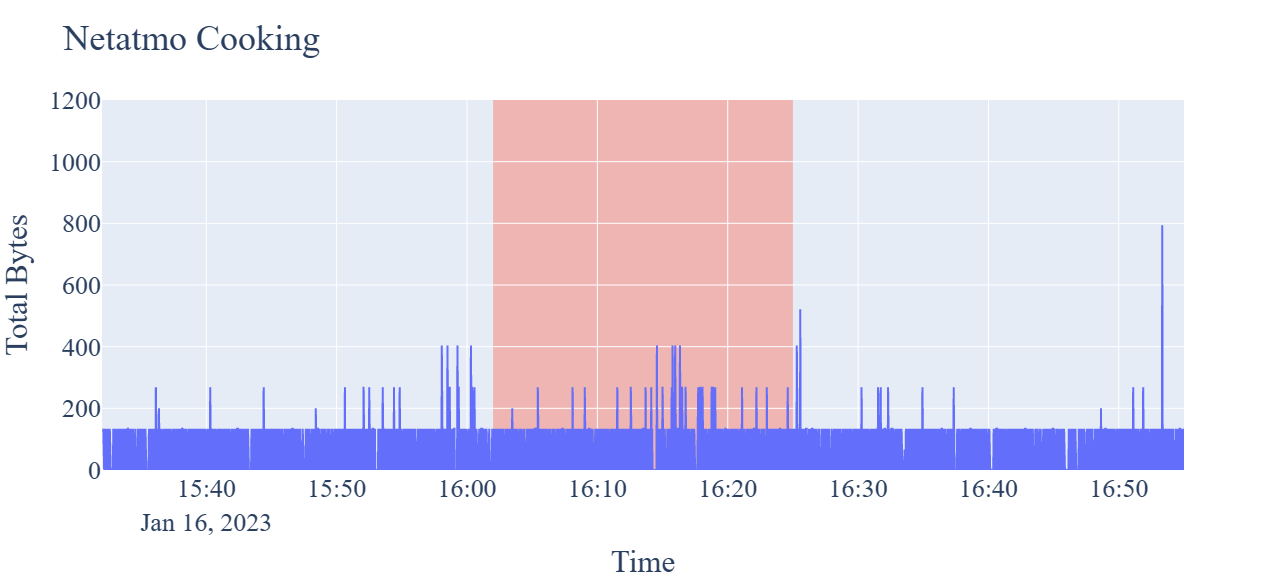
\includegraphics[width=1.2\hsize]{figures/Netatmo_Cooking_Bytes_16.01.png}
    \end{subfigure}
    \begin{subfigure}[b]{0.5\textwidth}
        \centering
        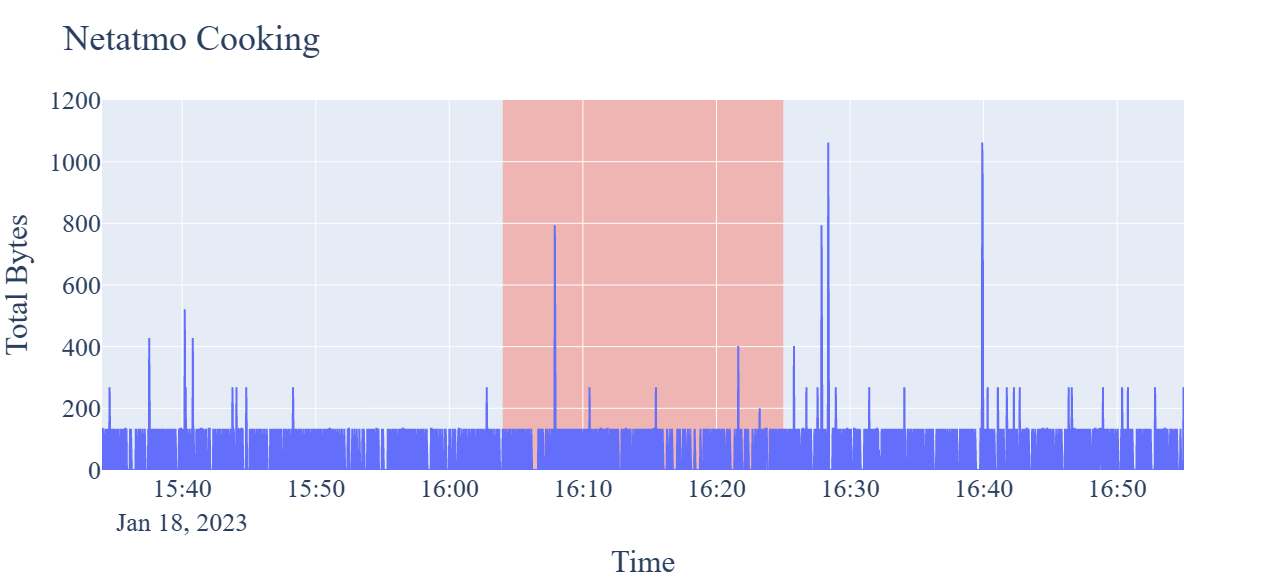
\includegraphics[width=1.2\hsize]{figures/Netatmo_Cooking_Bytes_18.01.png}
    \end{subfigure}
    \begin{subfigure}[b]{0.5\textwidth}
        \centering
        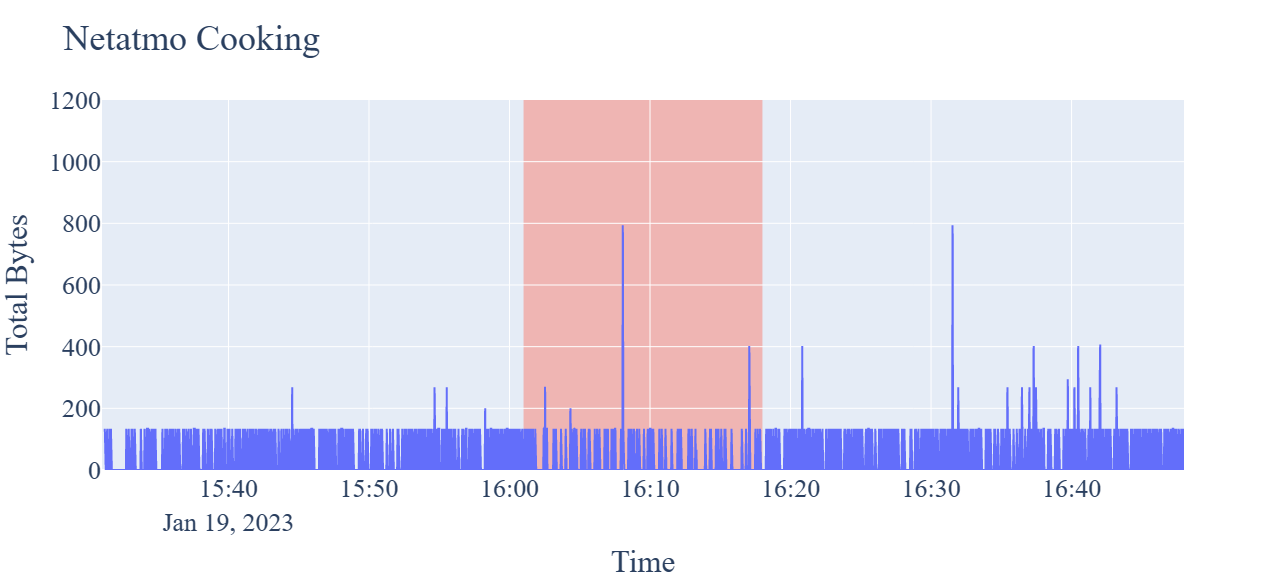
\includegraphics[width=1.2\hsize]{figures/Netatmo_Cooking_Bytes_19.01.png}
    \end{subfigure}
    \begin{subfigure}[b]{0.5\textwidth}
        \centering
        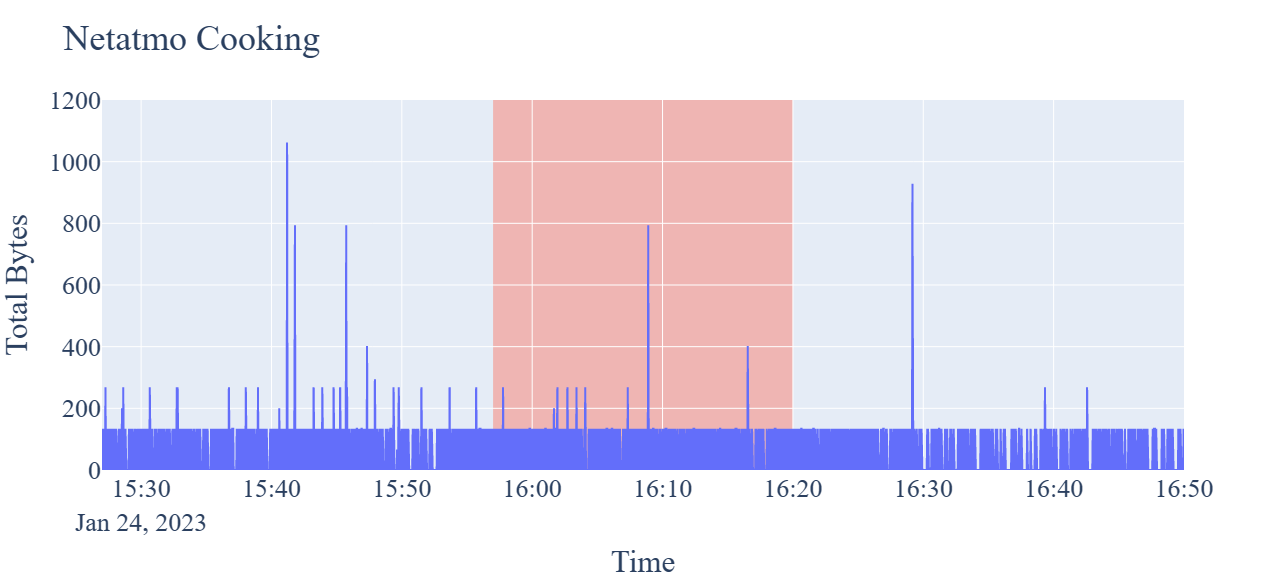
\includegraphics[width=1.2\hsize]{figures/Netatmo_Cooking_Bytes_24.01.png}
    \end{subfigure}
    \begin{subfigure}[b]{0.5\textwidth}
        \centering
        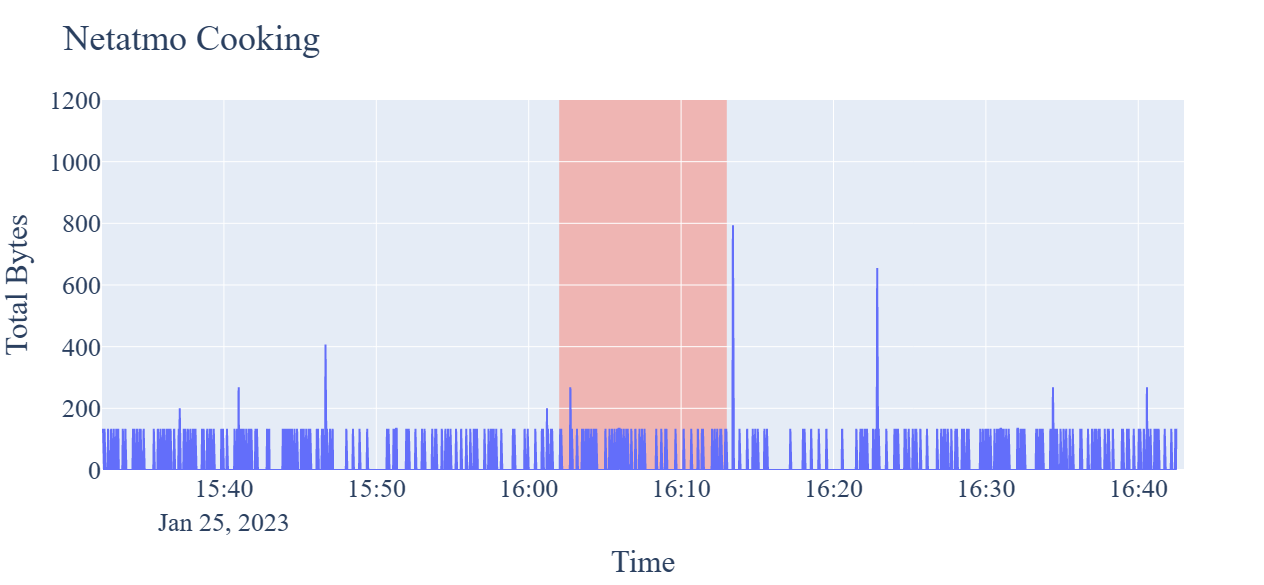
\includegraphics[width=1.2\hsize]{figures/Netatmo_Cooking_Bytes_25.01.png}
    \end{subfigure}
    \begin{subfigure}[b]{0.5\textwidth}
        \centering
        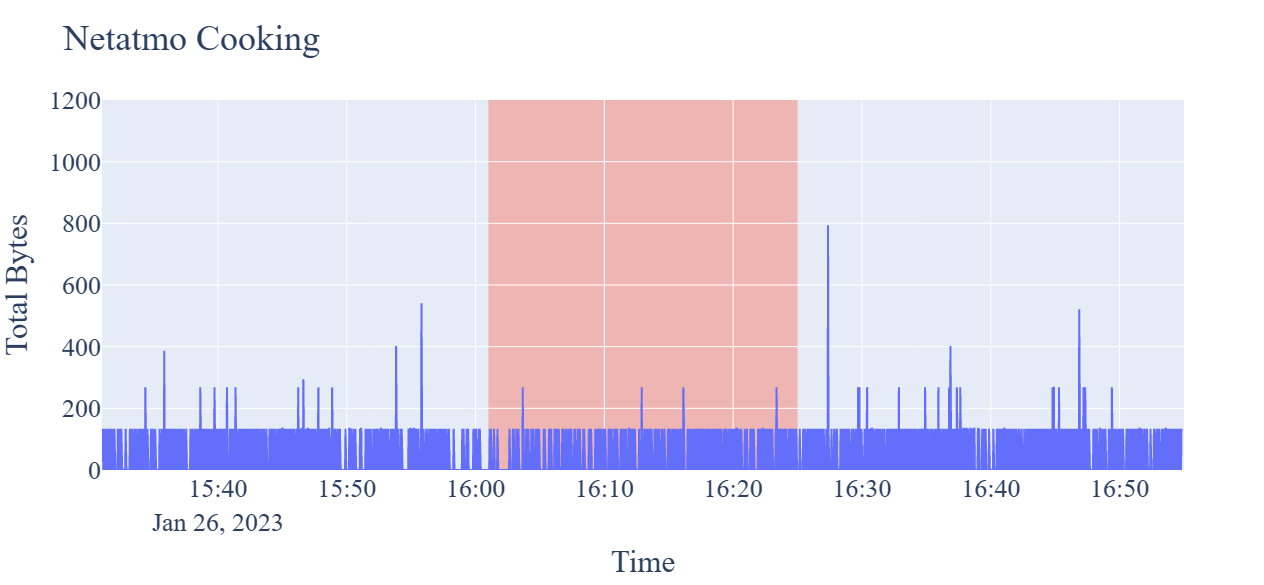
\includegraphics[width=1.2\hsize]{figures/Netatmo_Cooking_Bytes_26.01.png}
    \end{subfigure}
    \begin{subfigure}[b]{0.5\textwidth}
        \centering
        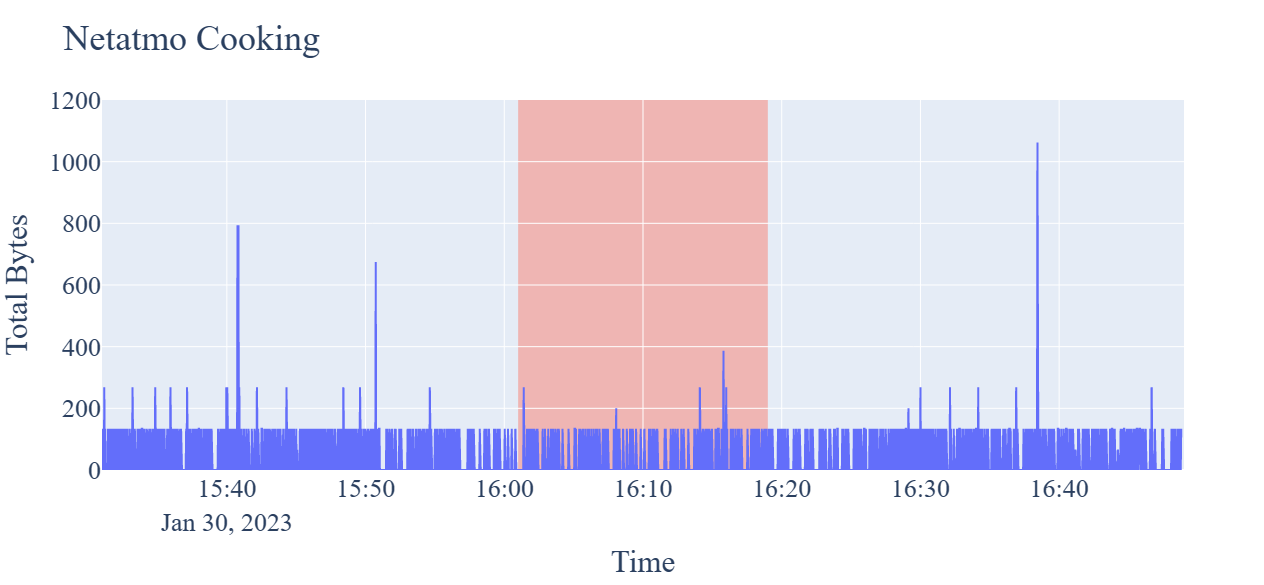
\includegraphics[width=1.2\hsize]{figures/Netatmo_Cooking_Bytes_30.01.png}
    \end{subfigure}
    \caption{Netatmo Cooking Events - Bytes}
    \label{fig:NetatmoCookingBytes}
\end{figure}

\begin{figure}[H]
    \begin{subfigure}[b]{0.5\textwidth}
        \centering
        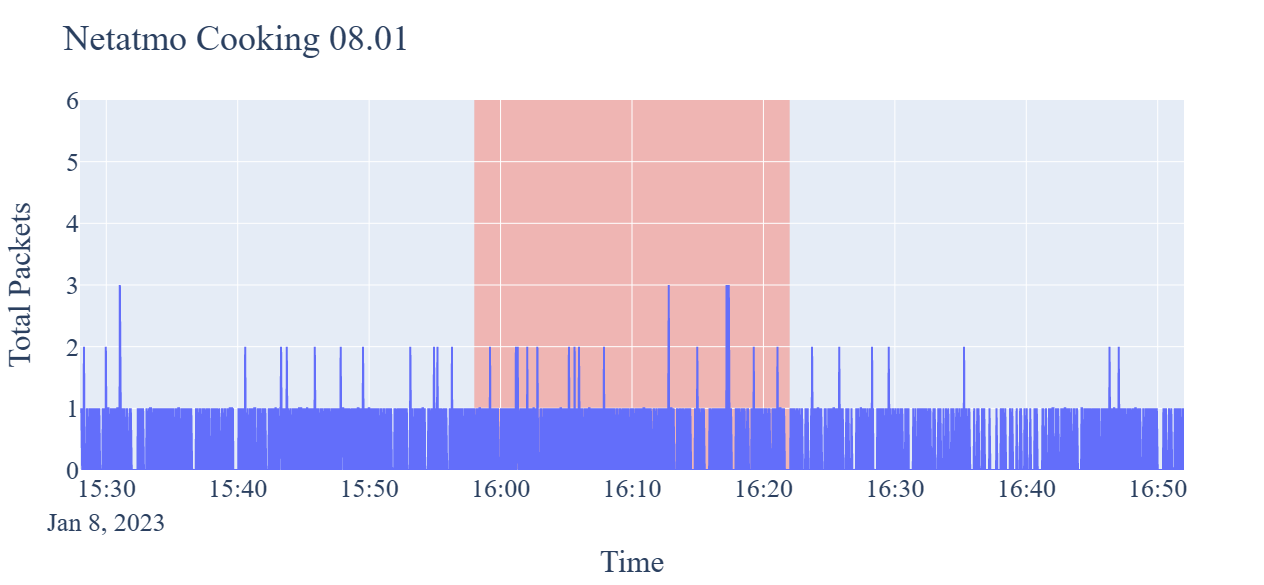
\includegraphics[width=1.2\hsize]{figures/Netatmo_Cooking_Packets_08.01.png}
    \end{subfigure}
    \begin{subfigure}[b]{0.5\textwidth}
        \centering
        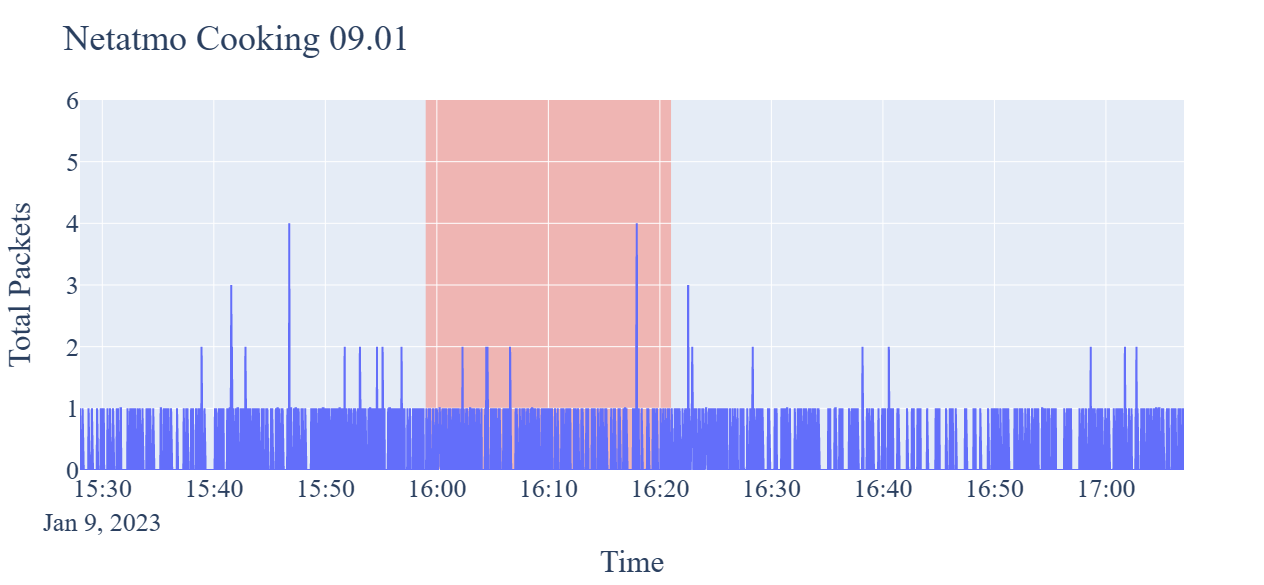
\includegraphics[width=1.2\hsize]{figures/Netatmo_Cooking_Packets_09.01.png}
    \end{subfigure}
    \begin{subfigure}[b]{0.5\textwidth}
        \centering
        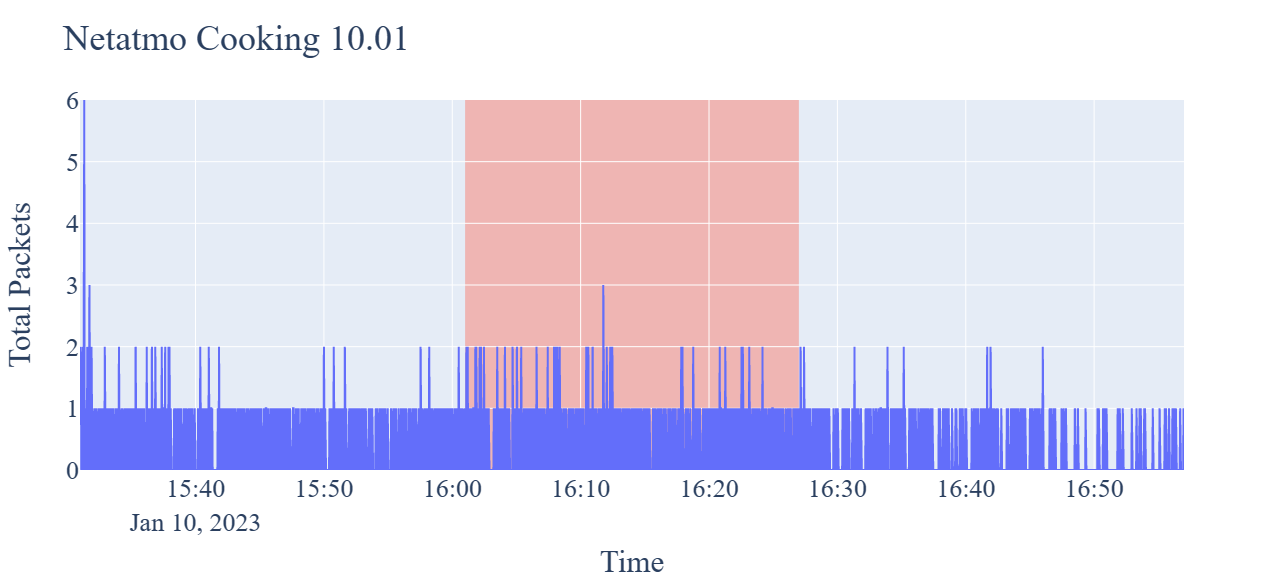
\includegraphics[width=1.2\hsize]{figures/Netatmo_Cooking_Packets_10.01.png}
    \end{subfigure}
    \begin{subfigure}[b]{0.5\textwidth}
        \centering
        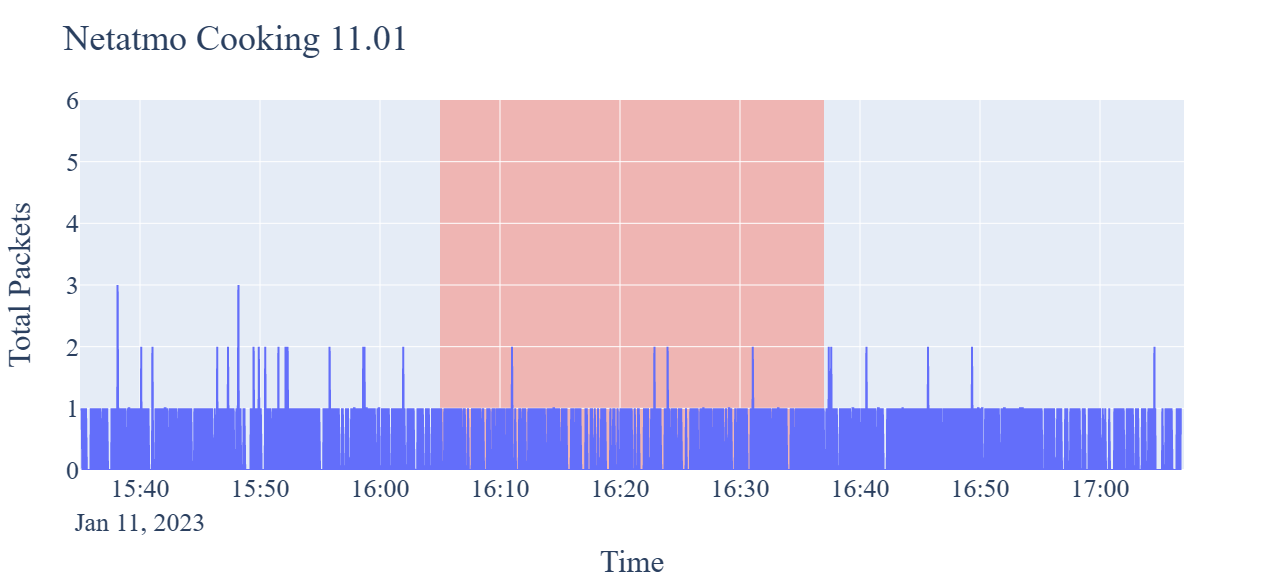
\includegraphics[width=1.2\hsize]{figures/Netatmo_Cooking_Packets_11.01.png}
    \end{subfigure}
    \begin{subfigure}[b]{0.5\textwidth}
        \centering
        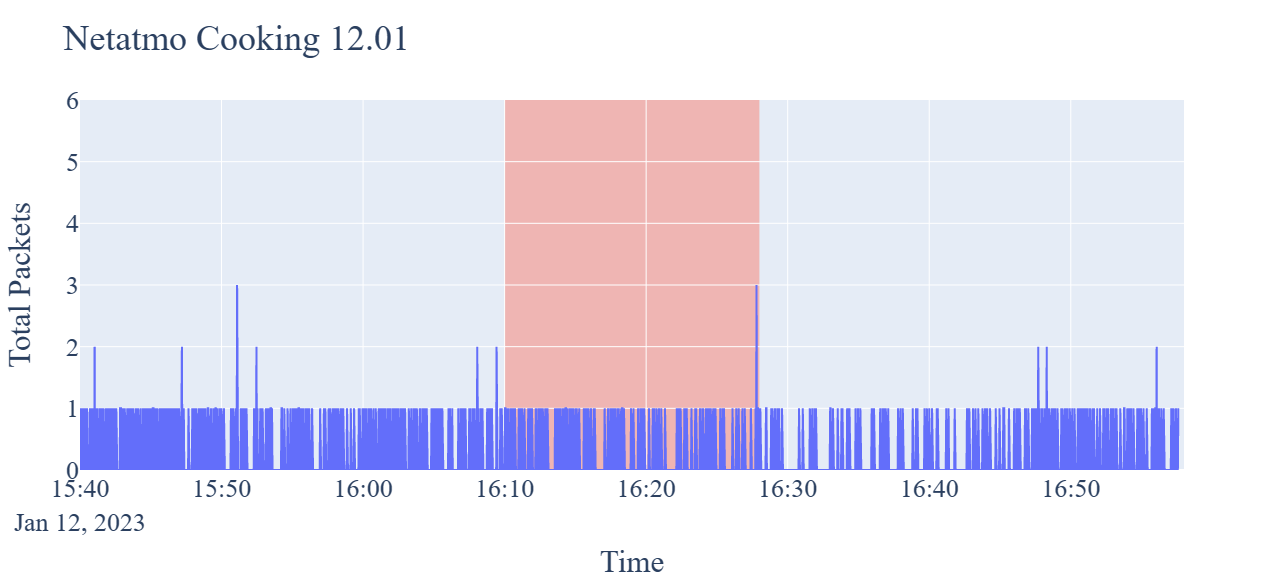
\includegraphics[width=1.2\hsize]{figures/Netatmo_Cooking_Packets_12.01.png}
    \end{subfigure}
    \begin{subfigure}[b]{0.5\textwidth}
        \centering
        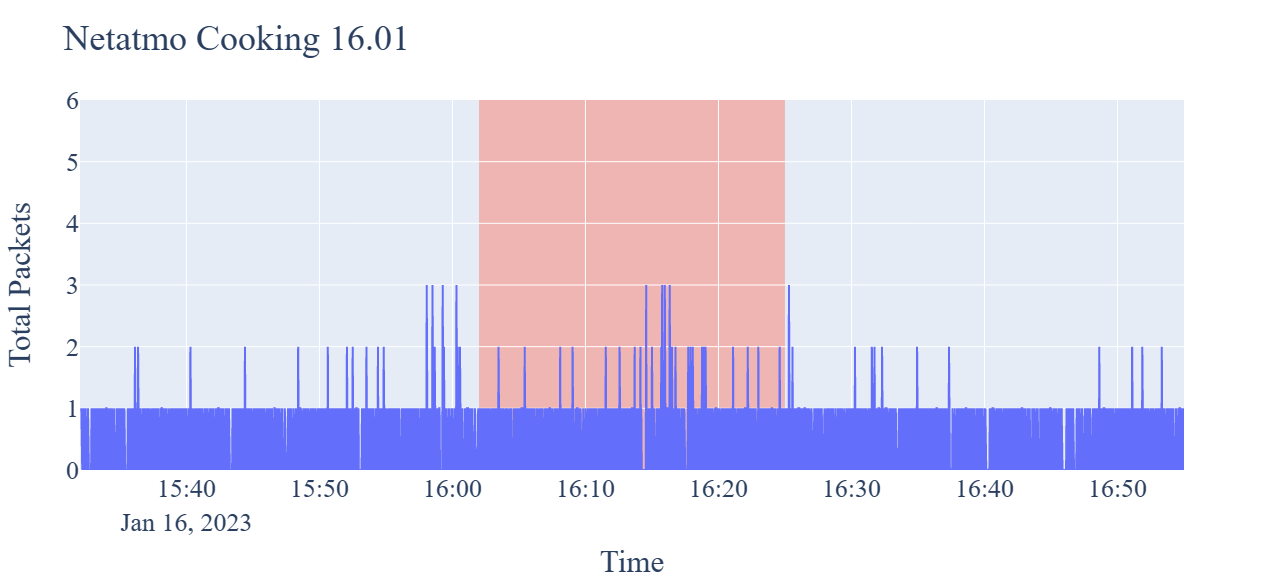
\includegraphics[width=1.2\hsize]{figures/Netatmo_Cooking_Packets_16.01.png}
    \end{subfigure}
    \begin{subfigure}[b]{0.5\textwidth}
        \centering
        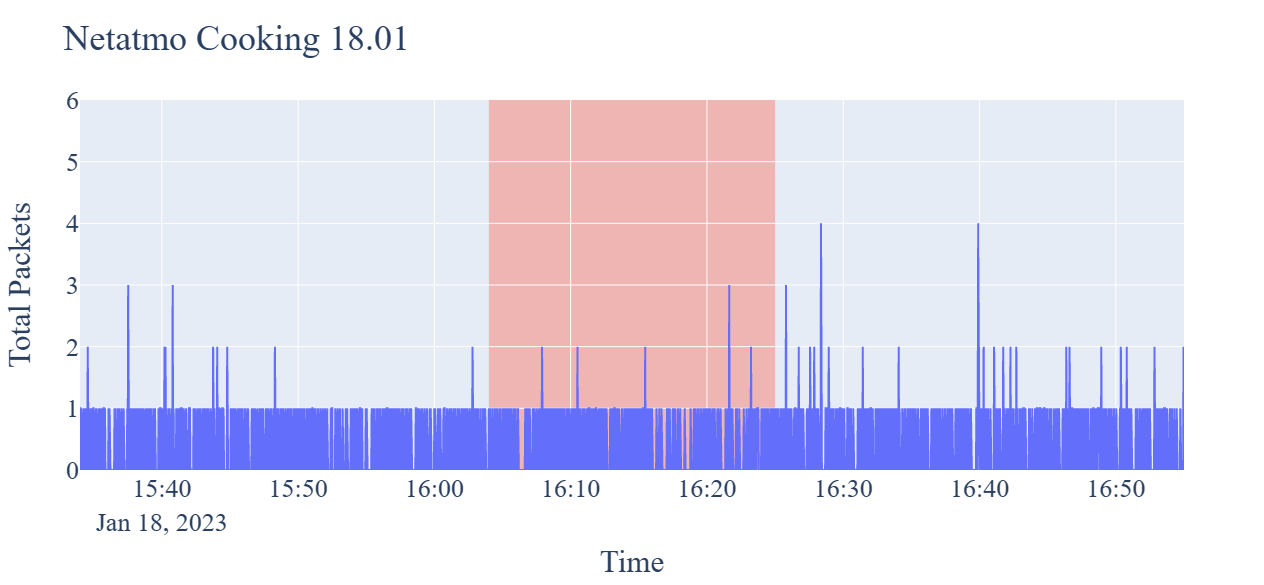
\includegraphics[width=1.2\hsize]{figures/Netatmo_Cooking_Packets_18.01.png}
    \end{subfigure}
    \begin{subfigure}[b]{0.5\textwidth}
        \centering
        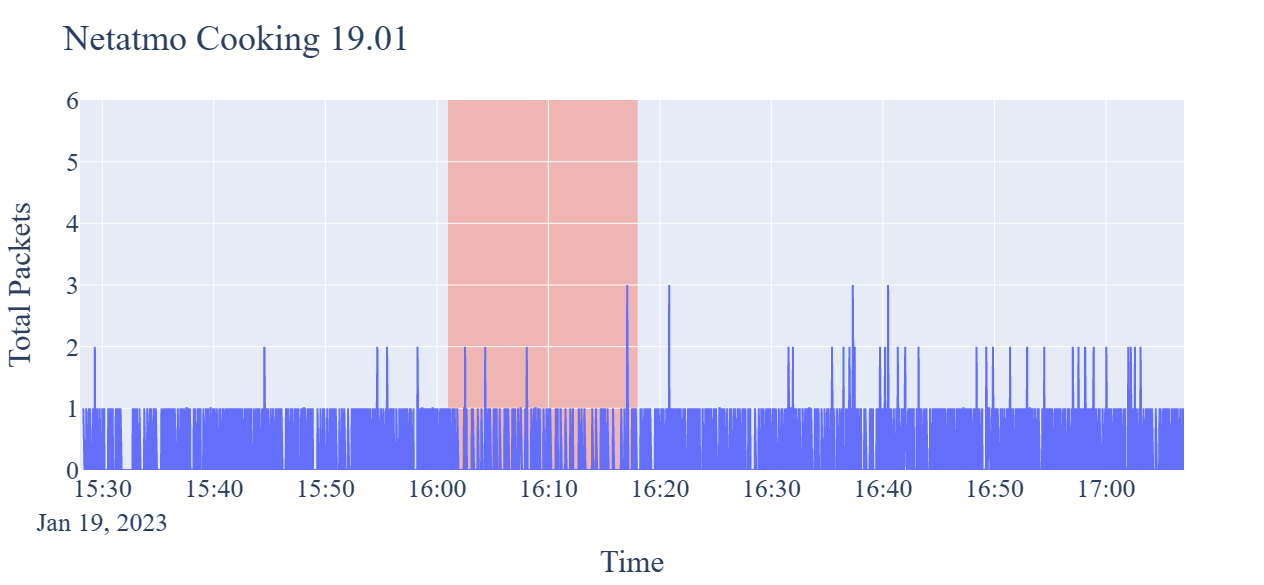
\includegraphics[width=1.2\hsize]{figures/Netatmo_Cooking_Packets_19.01.png}
    \end{subfigure}
    \begin{subfigure}[b]{0.5\textwidth}
        \centering
        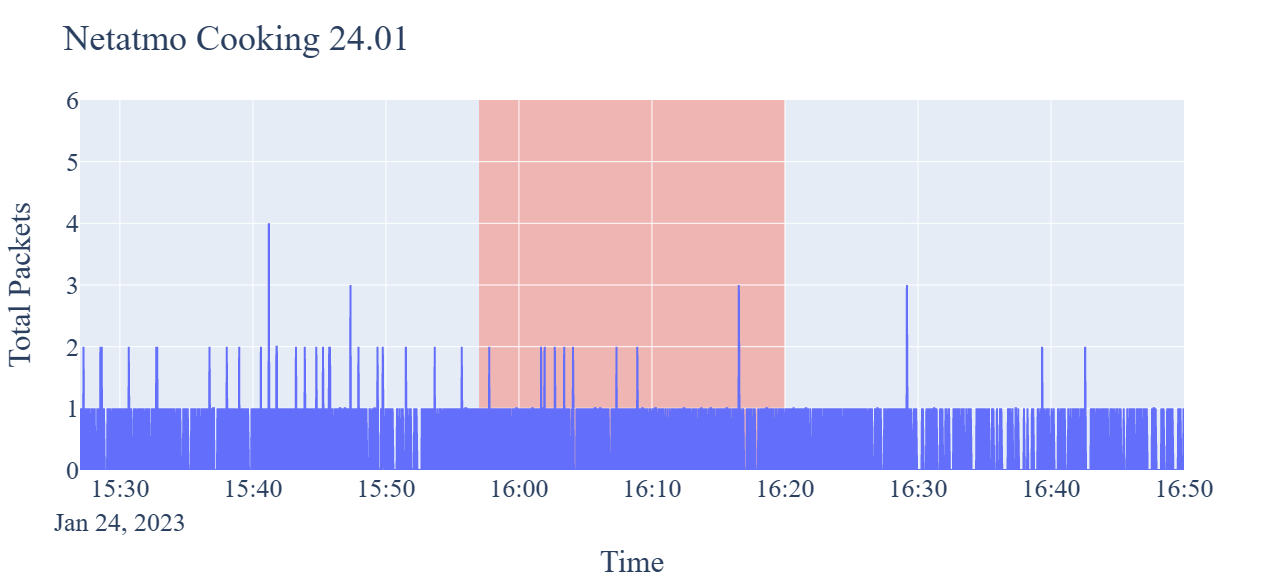
\includegraphics[width=1.2\hsize]{figures/Netatmo_Cooking_Packets_24.01.png}
    \end{subfigure}
    \begin{subfigure}[b]{0.5\textwidth}
        \centering
        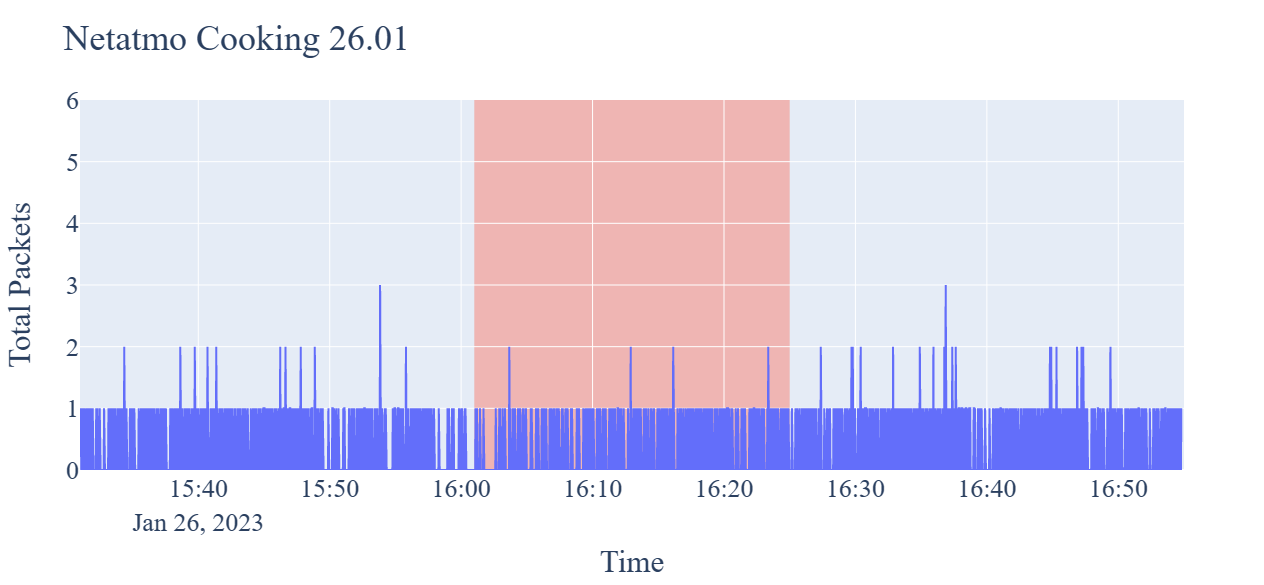
\includegraphics[width=1.2\hsize]{figures/Netatmo_Cooking_Packets_26.01.png}
    \end{subfigure}
    \begin{subfigure}[b]{0.5\textwidth}
        \centering
        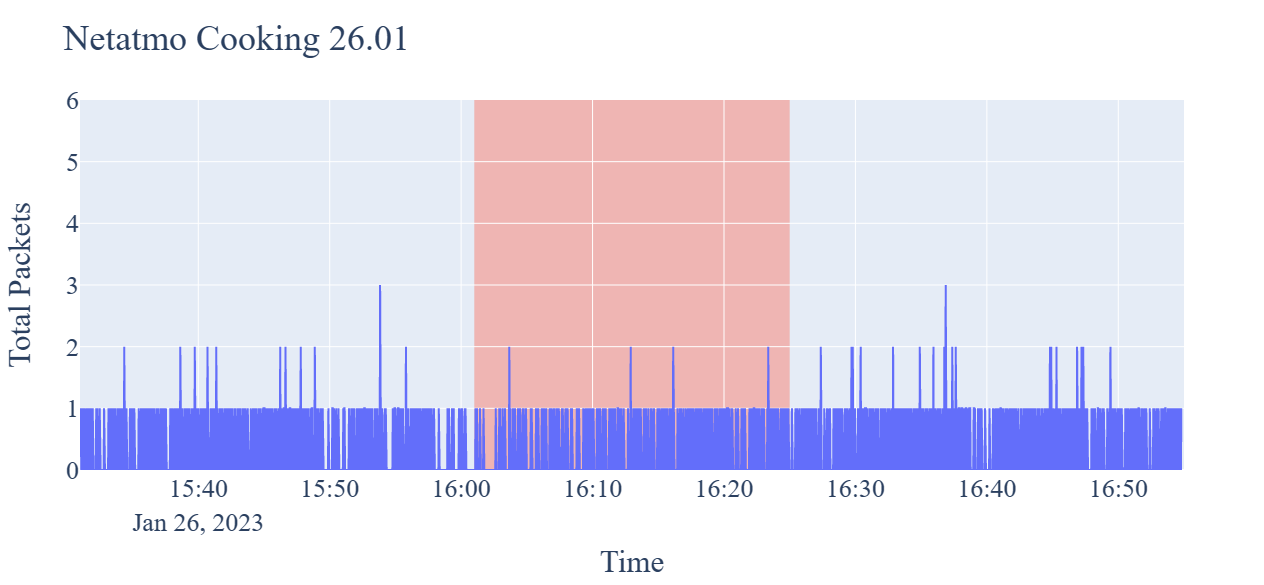
\includegraphics[width=1.2\hsize]{figures/Netatmo_Cooking_Packets_26.01.png}
    \end{subfigure}
    \begin{subfigure}[b]{0.5\textwidth}
        \centering
        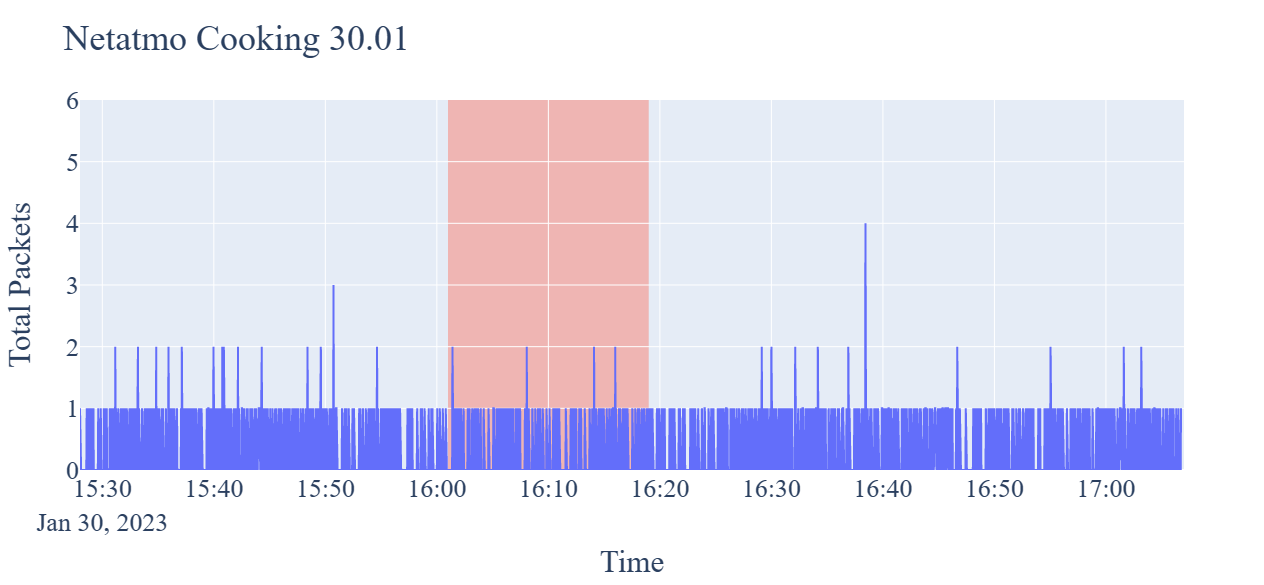
\includegraphics[width=1.2\hsize]{figures/Netatmo_Cooking_Packets_30.01.png}
    \end{subfigure}
    \caption{Netatmo Cooking Events - Packets}
    \label{fig:NetatmoCookingPackets}
\end{figure}

It is hard to see any specific changes in the traffic flow from when the event is ongoing based on the graphs given in figure \ref{fig:NetatmoCookingBytes} and \ref{fig:NetatmoCookingPackets}. Also looking at the table \ref{tab:NetatmoCookingCalculations} the calculations varies a lot. From table \ref{tab:NetatmoCookingCalculations}, the packets varies from 309 to 921 packets and from 42,332 to 123,899 bytes. 
\\\\
The next step is to compare the event graphs and calculations with the baseline traffic from the correlating timing for cooking events. Figure \ref{fig:NetatmoCookingComparingBytes} and \ref{fig:NetatmoCookingComparingPackets} compares the graphs for cooking from the actual events, marked in red, to the baseline capture, marked in blue. 

\begin{figure}[H]
    \begin{subfigure}[b]{0.47\textwidth}
        \centering
        \tcbincludegraphics[size=fbox,width=1.1\hsize,colframe=red]{figures/Netatmo_Cooking_Packets_08.01.png}
    \end{subfigure}
    \begin{subfigure}[b]{0.47\textwidth}
        \centering
        \tcbincludegraphics[size=fbox,width=1.1\hsize, colframe=blue]{figures/Netatmo_Cooking_Baseline_Packets_06.03.png}
    \end{subfigure}
    \begin{subfigure}[b]{0.47\textwidth}
        \centering
        \tcbincludegraphics[size=fbox,width=1.1\hsize,colframe=red]{figures/Netatmo_Cooking_Packets_10.01.png}
    \end{subfigure}
    \begin{subfigure}[b]{0.47\textwidth}
        \centering
        \tcbincludegraphics[size=fbox,width=1.1\hsize,colframe=blue]{figures/Netatmo_Cooking_Baseline_Packets_07.03.png}
    \end{subfigure}
    \begin{subfigure}[b]{0.47\textwidth}
        \centering
        \tcbincludegraphics[size=fbox,width=1.1\hsize,colframe=red]{figures/Netatmo_Cooking_Packets_12.01.png}
    \end{subfigure}
    \begin{subfigure}[b]{0.47\textwidth}
        \centering
        \tcbincludegraphics[size=fbox,width=1.1\hsize,colframe=blue]{figures/Netatmo_Cooking_Baseline_Packets_08.03.png}
    \end{subfigure}
    \begin{subfigure}[b]{0.47\textwidth}
        \centering
        \tcbincludegraphics[size=fbox,width=1.1\hsize,colframe=red]{figures/Netatmo_Cooking_Packets_18.01.png}
    \end{subfigure}
    \begin{subfigure}[b]{0.47\textwidth}
        \centering
        \tcbincludegraphics[size=fbox,width=1.1\hsize,colframe=blue]{figures/Netatmo_Cooking_Baseline_Packets_09.03.png}
    \end{subfigure}
    \begin{subfigure}[b]{0.47\textwidth}
        \centering
        \tcbincludegraphics[size=fbox,width=1.1\hsize,colframe=red]{figures/Netatmo_Cooking_Packets_24.01.png}
    \end{subfigure}
    \begin{subfigure}[b]{0.47\textwidth}
        \centering
        \tcbincludegraphics[size=fbox,width=1.1\hsize,colframe=blue]{figures/Netatmo_Cooking_Baseline_Packets_10.03.png}
    \end{subfigure}
        \begin{subfigure}[b]{0.47\textwidth}
        \centering
        \tcbincludegraphics[size=fbox,width=1.1\hsize,colframe=red]{figures/Netatmo_Cooking_Packets_26.01.png}
    \end{subfigure}
    \begin{subfigure}[b]{0.47\textwidth}
        \centering
        \tcbincludegraphics[size=fbox,width=1.1\hsize,colframe=blue]{figures/Netatmo_Cooking_Baseline_Packets_11.03.png}
    \end{subfigure}
    \begin{subfigure}[b]{0.47\textwidth}
        \centering
        \tcbincludegraphics[size=fbox,width=1.1\hsize,colframe=red]{figures/Netatmo_Cooking_Packets_30.01.png}
    \end{subfigure}
    \hspace{0.6cm}
    \begin{subfigure}[b]{0.47\textwidth}
    \centering
        \tcbincludegraphics[size=fbox,width=1.1\hsize,colframe=blue]{figures/Netatmo_Cooking_Baseline_Packets_12.03.png}
        \end{subfigure}
    \caption{Comparing Events and Baseline Packets for Cooking - Netatmo}
    \label{fig:NetatmoCookingComparingPackets}
\end{figure}

\begin{figure}[H]
    \begin{subfigure}[b]{0.47\textwidth}
        \centering
        \tcbincludegraphics[size=fbox,width=1.1\hsize,colframe=red]{figures/Netatmo_Cooking_Bytes_08.01.png}
    \end{subfigure}
    \begin{subfigure}[b]{0.47\textwidth}
        \centering
        \tcbincludegraphics[size=fbox,width=1.1\hsize,colframe=blue]{figures/Netatmo_Cooking_Baseline_Bytes_06.03.png}
    \end{subfigure}
    \begin{subfigure}[b]{0.47\textwidth}
        \centering
        \tcbincludegraphics[size=fbox,width=1.1\hsize,colframe=red]{figures/Netatmo_Cooking_Bytes_10.01.png}
    \end{subfigure}
    \begin{subfigure}[b]{0.47\textwidth}
        \centering
        \tcbincludegraphics[size=fbox,width=1.1\hsize,colframe=blue]{figures/Netatmo_Cooking_Baseline_Bytes_07.03.png}
    \end{subfigure}
    \begin{subfigure}[b]{0.47\textwidth}
        \centering
        \tcbincludegraphics[size=fbox,width=1.1\hsize,colframe=red]{figures/Netatmo_Cooking_Bytes_12.01.png}
    \end{subfigure}
    \begin{subfigure}[b]{0.47\textwidth}
        \centering
        \tcbincludegraphics[size=fbox,width=1.1\hsize,colframe=blue]{figures/Netatmo_Cooking_Baseline_Bytes_08.03.png}
    \end{subfigure}
    \begin{subfigure}[b]{0.47\textwidth}
        \centering
        \tcbincludegraphics[size=fbox,width=1.1\hsize,colframe=red]{figures/Netatmo_Cooking_Bytes_18.01.png}
    \end{subfigure}
    \begin{subfigure}[b]{0.47\textwidth}
        \centering
        \tcbincludegraphics[size=fbox,width=1.1\hsize,colframe=blue]{figures/Netatmo_Cooking_Baseline_Bytes_09.03.png}
    \end{subfigure}
    \begin{subfigure}[b]{0.47\textwidth}
        \centering
        \tcbincludegraphics[size=fbox,width=1.1\hsize,colframe=red]{figures/Netatmo_Cooking_Bytes_24.01.png}
    \end{subfigure}
    \begin{subfigure}[b]{0.47\textwidth}
        \centering
        \tcbincludegraphics[size=fbox,width=1.1\hsize,colframe=blue]{figures/Netatmo_Cooking_Baseline_Bytes_10.03.png}
    \end{subfigure}
        \begin{subfigure}[b]{0.47\textwidth}
        \centering
        \tcbincludegraphics[size=fbox,width=1.1\hsize,colframe=red]{figures/Netatmo_Cooking_Bytes_26.01.png}
    \end{subfigure}
    \begin{subfigure}[b]{0.47\textwidth}
        \centering
        \tcbincludegraphics[size=fbox,width=1.1\hsize,colframe=blue]{figures/Netatmo_Cooking_Baseline_Bytes_11.03.png}
    \end{subfigure}
    \begin{subfigure}[b]{0.47\textwidth}
        \centering
        \tcbincludegraphics[size=fbox,width=1.1\hsize,colframe=red]{figures/Netatmo_Cooking_Bytes_30.01.png}
    \end{subfigure}
    \hspace{0.6cm}
    \begin{subfigure}[b]{0.47\textwidth}
    \centering
        \tcbincludegraphics[size=fbox,width=1.1\hsize,colframe=blue]{figures/Netatmo_Cooking_Baseline_Bytes_12.03.png}
        \end{subfigure}
    \caption{Comparing Events and Baseline Bytes for Cooking - Netatmo}
    \label{fig:NetatmoCookingComparingBytes}
\end{figure}

First comparing the graphs in figure \ref{fig:NetatmoCookingComparingBytes} and \ref{fig:NetatmoCookingComparingPackets} it is not possible to see distinct differences in the red graphs from the actual events to the blue graphs from the baseline. Calculations on the baseline cooking pcaps has been made to compare even further with the event. In table \ref{tab:NetatmoBaselineCookingCalculations} the same calculations as the event had, are presented. In table \ref{tab:NetatmoComparingBaselineAndCookingCalculations} a comparison between the average values from both the baseline and the events are summarized. At last, a graphical comparison of bytes and packets from the event and baseline are given in figure \ref{fig:NetatmoComparingCookingCalculations}. 

\begin{table}[!ht]
    \centering
    \caption{Netatmo Baseline Cooking Calculations}
    \begin{tabular}{|l|l|l|l|l|l|}
    \hline
        \textbf{Baseline} & \textbf{Packets} & \textbf{Bytes} & \textbf{Biggest packet} & \textbf{Average bytes/s} & \textbf{Average packet size} \\ \hline
        06.mar & 475 & 63,242 & 134 & 13 & 133 bytes\\ \hline
        07.mar & 793 & 108,478 & 407 & 22 & 137 bytes\\ \hline
        08.mar & 573 & 77,841 & 407 & 16 & 136 bytes \\ \hline
        09.mar & 685 & 92,265 & 407 & 19 & 135 bytes \\ \hline
        10.mar & 666 & 89,962 & 407 & 18 & 135 bytes \\ \hline
        11.mar & 539 & 73,745 & 407 & 15 & 137 bytes \\ \hline
        12.mar & 497 & 66,464 & 136 & 14 & 134 bytes \\ \hline
        13.mar & 636 & 84,750 & 136 & 17 & 133 bytes \\ \hline
        14.mar & 570 & 78,412 & 407 & 16 & 138 bytes \\ \hline
        15.mar & 674 & 90,275 & 407 & 19 & 134 bytes \\ \hline
        \textbf{Average} &  \textbf{611}  &  \textbf{82,543}  &  \textbf{326}  &  \textbf{17}  &  \textbf{135 bytes}  \\ \hline
        \textbf{Std dev}  &  \textbf{98}   &  \textbf{13,476}   &  \textbf{131}   &  \textbf{3}   &  \textbf{2 bytes}   \\ \hline
    \end{tabular}
    \label{tab:NetatmoBaselineCookingCalculations}
\end{table}

\begin{table}[H]
    \centering
    \caption{Comparing Cooking and Baseline Calculations for Netatmo}
    \begin{tabular}{|l|l|l|l|l|}
    \hline
        \textbf{} & \textbf{Event average} & \textbf{Event std dev} & \textbf{Baseline average} & \textbf{Baseline std dev} \\ \hline
        Packets  &  687  &  147   &  611  &  98  \\ \hline
        Bytes  &  93,821  &  19,914   &  82,543  &  13,476   \\ \hline
        Biggest packet  &  375  &  85   &  326  &  131   \\ \hline
        Average bytes/s  &  19  &  3   &  17  &  3   \\ \hline
        Average packet size  &  136 bytes  &  1 bytes  &  135 bytes &  2 bytes  \\ \hline
    \end{tabular}
    \label{tab:NetatmoComparingBaselineAndCookingCalculations}
\end{table}

\begin{figure}[H]
    \centering
    \begin{subfigure}{0.49\textwidth}
        \centering
        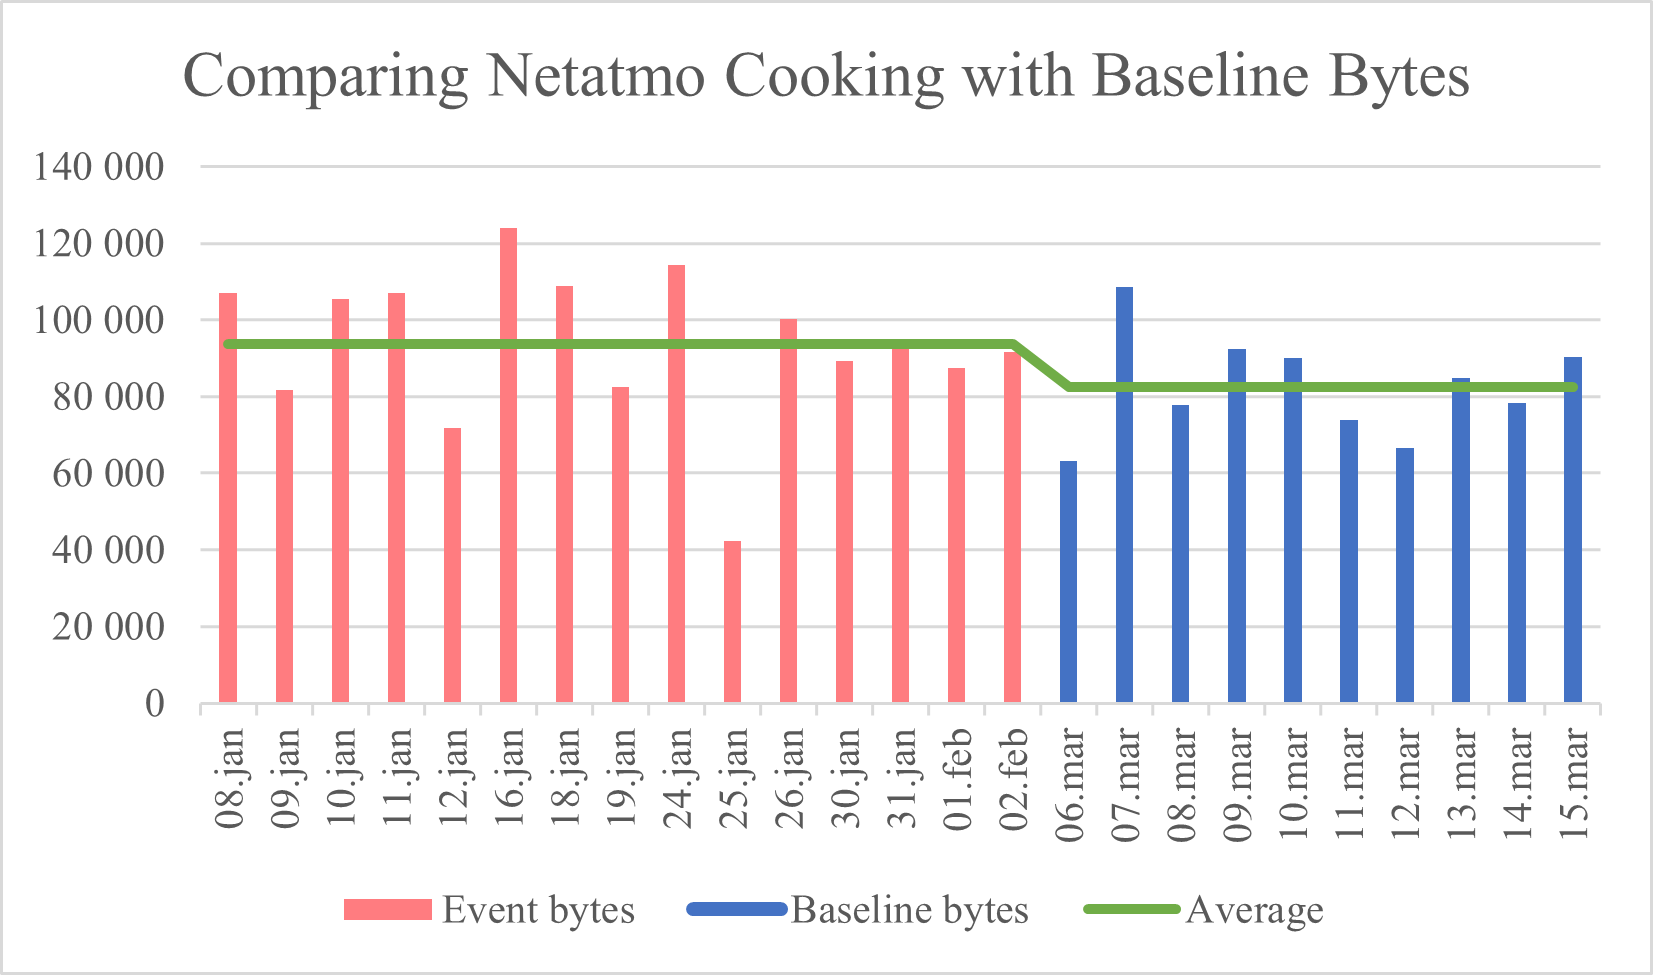
\includegraphics[width=1\hsize]{figures/Netatmo_Comparing_Cooking_Calculations_Bytes.png} 
    \end{subfigure}
    \begin{subfigure}{0.49\textwidth}
        \centering
        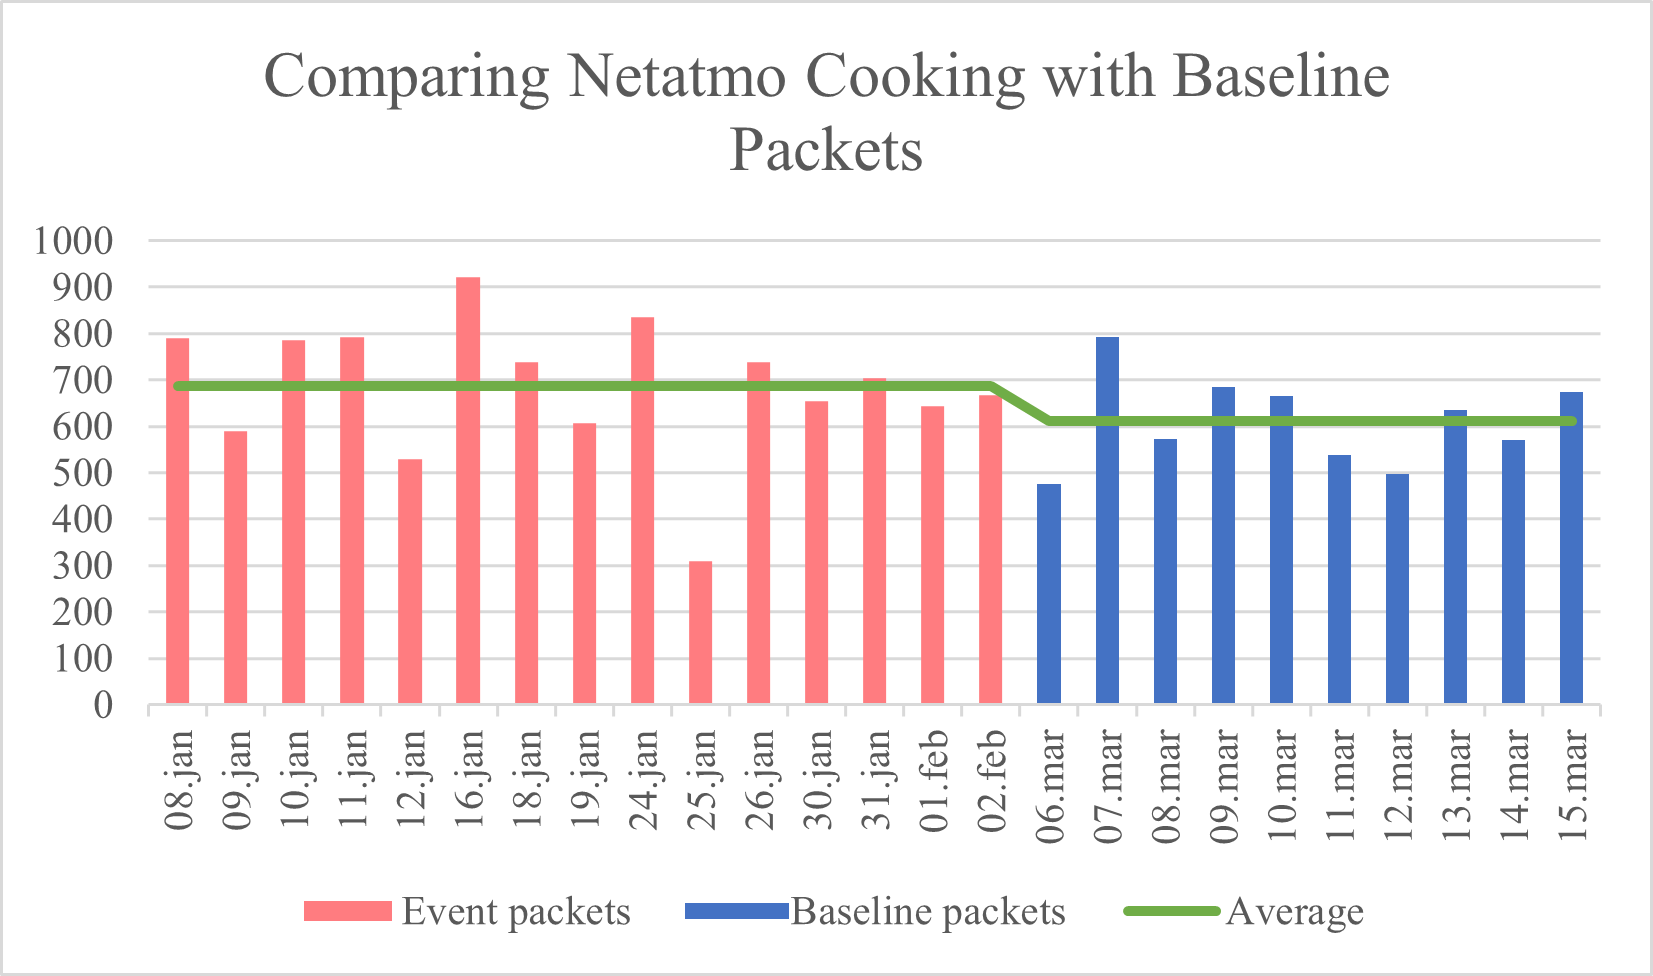
\includegraphics[width=1\hsize]{figures/Netatmo_Comparing_Cooking_Calculations_Packets.png} 
    \end{subfigure}
    \caption{Comparing Cooking Calculations for Netatmo}
    \label{fig:NetatmoComparingCookingCalculations}
\end{figure}

\subsection{Mill Sense}
The graphs in figure \ref{fig:NetatmoCookingBytes} and \ref{fig:MillCookingPackets} shows both bytes and packets for the first 10 of the cooking events. The area marked red on the graphs are when the event was ongoing. Table \ref{tab:MillCookingCalculations} presents the calculations from all the 15 cooking events. 

\begin{table}[!ht]
    \centering
    \caption{Mill Cooking Calculations}
    \begin{tabular}{|l|l|l|l|l|l|}
    \hline
        \textbf{Events} & \textbf{Packets} & \textbf{Bytes} & \textbf{Biggest packet} & \textbf{Average bytes/s} & \textbf{Average packet size } \\ \hline
        08.jan & 7,729 & 945,461 & 456 bytes & 189 & 122 bytes \\ \hline
        09.jan & 6,328 & 863,911 & 456 bytes & 177 & 137 bytes \\ \hline
        10.jan & 6,821 & 916,827 & 456 bytes & 179 & 134 bytes \\ \hline
        11.jan & 9,457 & 1,218,558 & 456 bytes & 223 & 129 bytes \\ \hline
        12.jan & 7,600 & 965,797 & 456 bytes & 208 & 127 bytes \\ \hline
        16.jan & 8,416 & 1,155,609 & 1,353 bytes & 234 & 137 bytes \\ \hline
        18.jan & 7,589 & 938,903 & 456 bytes & 195 & 124 bytes \\ \hline
        19.jan & 7,075 & 872,150 & 1,593 bytes & 191 & 123 bytes \\ \hline
        24.jan & 9,395 & 1,129,302 & 1,593 bytes & 229 & 120 bytes \\ \hline
        25.jan & 5,818 & 734,000 & 1,583 bytes & 174 & 126 bytes \\ \hline
        26.jan & 8,240 & 1,056,828 & 1,593 bytes & 212 & 128 bytes \\ \hline
        30.jan & 9,285 & 1,067,084 & 456 & 230 & 115 bytes \\ \hline
        31.jan & 8,623 & 991,377 & 456 & 209 & 115 bytes \\ \hline
        01.feb & 8,678 & 1,026 864 & 456 & 216 & 118 bytes \\ \hline
        02.feb & 7,764 & 951,239 & 456 & 200 & 123 bytes \\ \hline
        \textbf{Average} & \textbf{7921} & \textbf{988927} & \textbf{818} & \textbf{204} & \textbf{125 bytes}  \\ \hline
        \textbf{Std dev} & \textbf{1101} & \textbf{124838} & \textbf{533} & \textbf{20} & \textbf{7 bytes}  \\ \hline
    \end{tabular}
    \label{tab:MillCookingCalculations}
\end{table}

\begin{figure}[H]
    \centering
    \begin{subfigure}{0.49\textwidth}
        \centering
        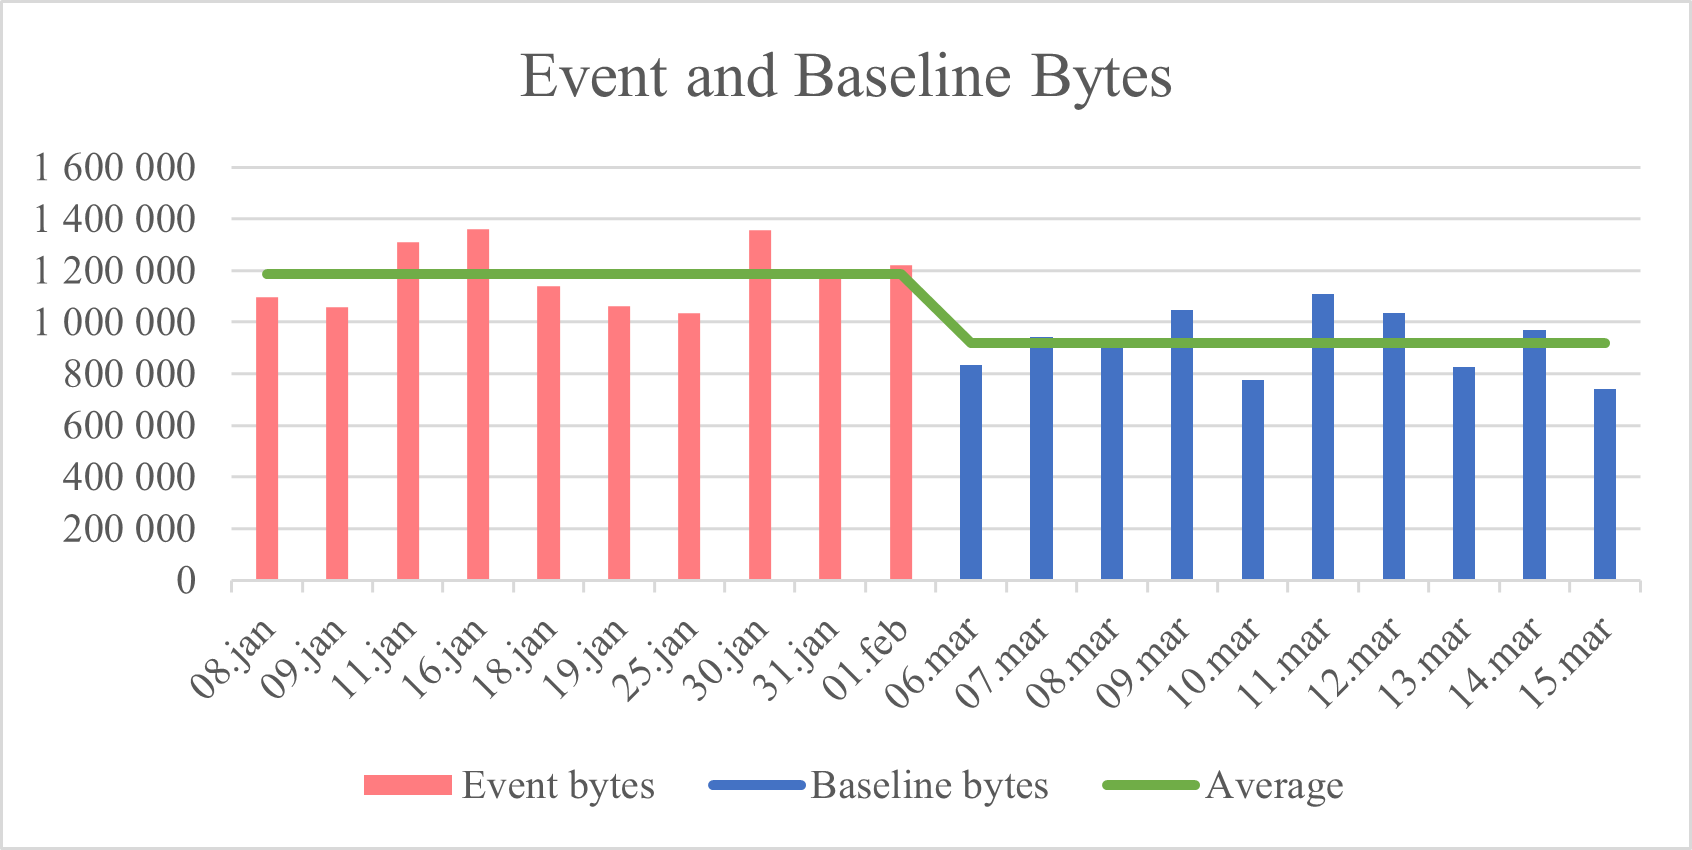
\includegraphics[width=1\hsize]{figures/Mill_Cooking_Calculations_Bytes.png} 
    \end{subfigure}
    \begin{subfigure}{0.49\textwidth}
        \centering
        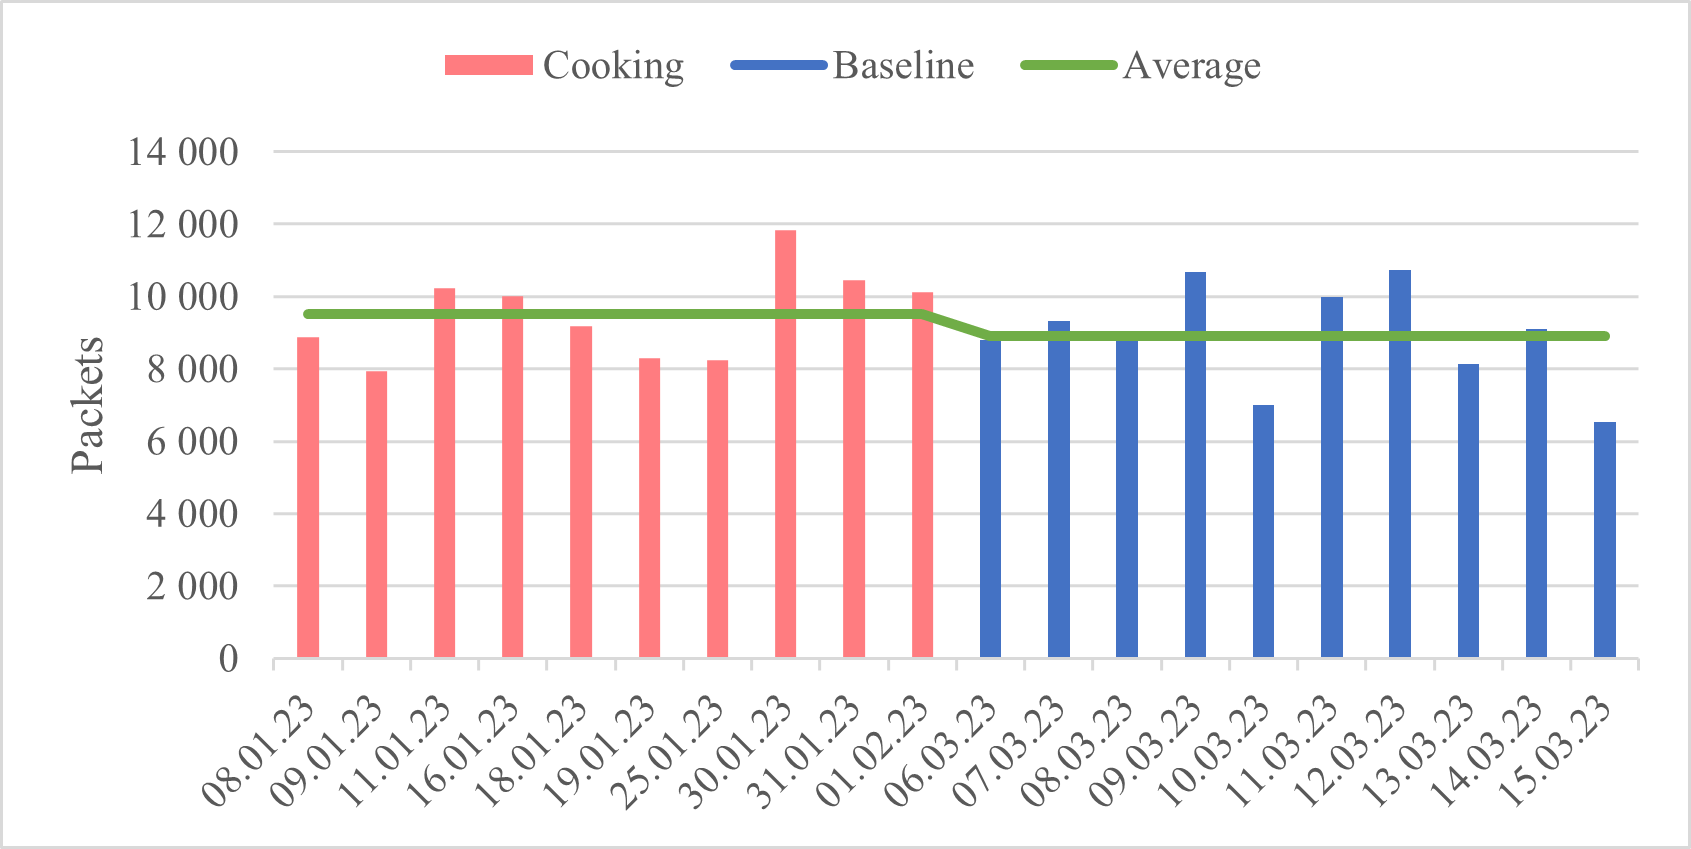
\includegraphics[width=1\hsize]{figures/Mill_Cooking_Calculations_Packets.png} 
    \end{subfigure}
    \caption{Cooking Calculations for Mill}
    \label{fig:MillComparingCookingCalculations}
\end{figure}

\begin{figure}[H]
    \begin{subfigure}[b]{0.5\textwidth}
        \centering
        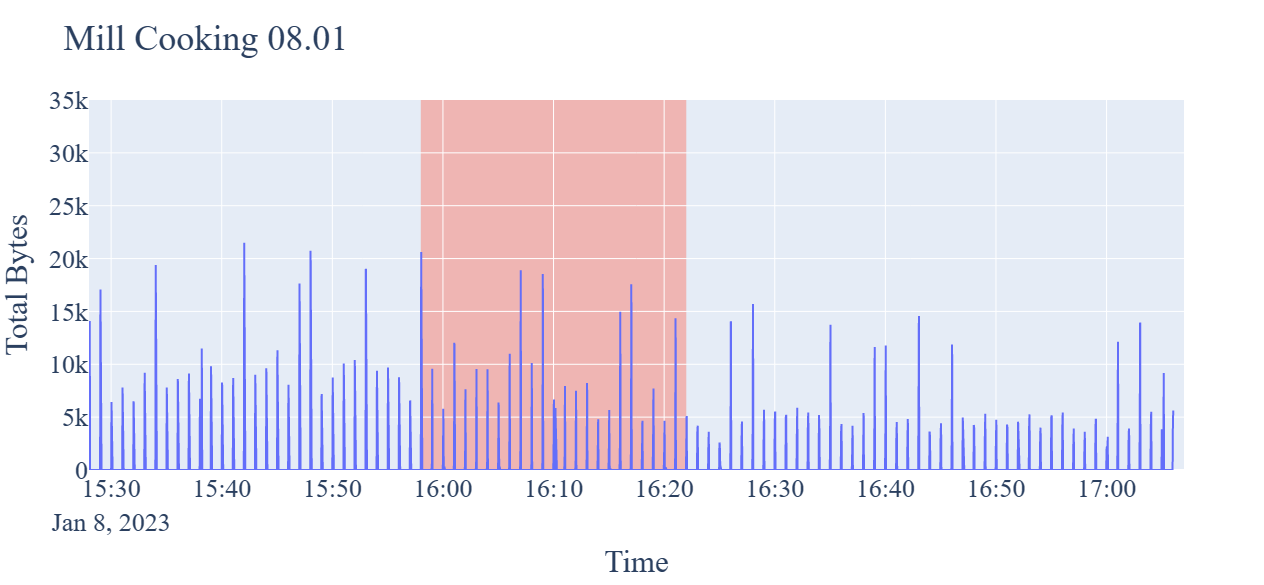
\includegraphics[width=1.2\hsize]{figures/Mill_Cooking_Bytes_08.01.png}
    \end{subfigure}
    \begin{subfigure}[b]{0.5\textwidth}
        \centering
        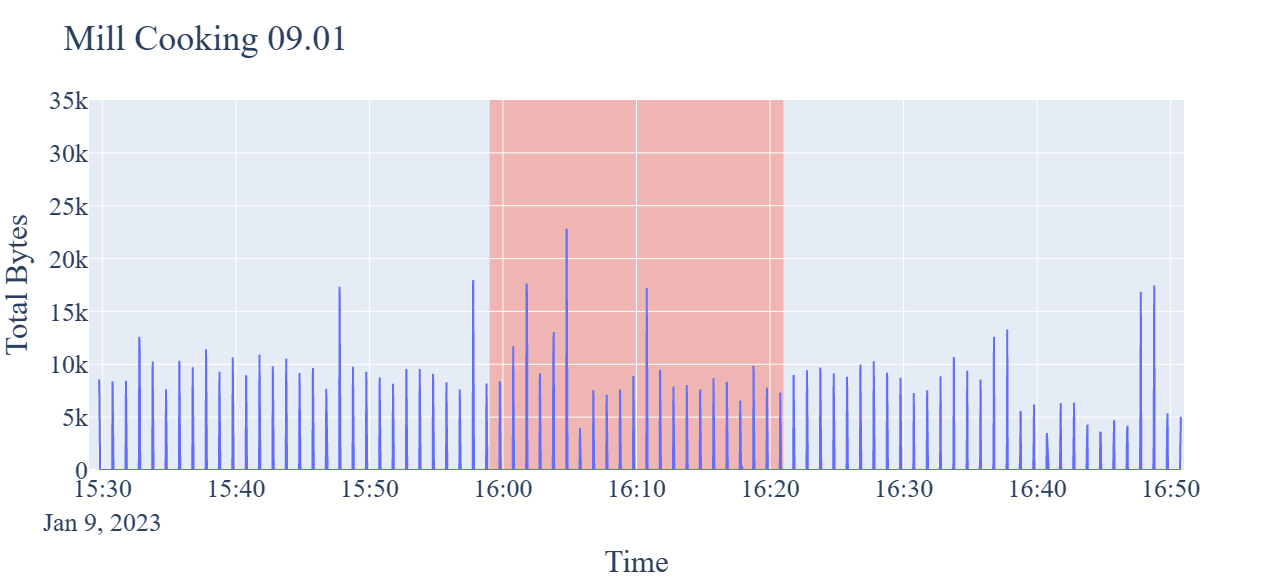
\includegraphics[width=1.2\hsize]{figures/Mill_Cooking_Bytes_09.01.png}
    \end{subfigure}
    \begin{subfigure}[b]{0.5\textwidth}
        \centering
        \includegraphics[width=1.2\hsize]{figures/Mill_Cooking_Bytes_10.01.png}
    \end{subfigure}
    \begin{subfigure}[b]{0.5\textwidth}
        \centering
        \includegraphics[width=1.2\hsize]{figures/Mill_Cooking_Bytes_11.01.png}
    \end{subfigure}
    \begin{subfigure}[b]{0.5\textwidth}
        \centering
        \includegraphics[width=1.2\hsize]{figures/Mill_Cooking_Bytes_12.01.png}
    \end{subfigure}
    \begin{subfigure}[b]{0.5\textwidth}
        \centering
        \includegraphics[width=1.2\hsize]{figures/Mill_Cooking_Bytes_16.01.png}
    \end{subfigure}
    \begin{subfigure}[b]{0.5\textwidth}
        \centering
        \includegraphics[width=1.2\hsize]{figures/Mill_Cooking_Bytes_18.01.png}
    \end{subfigure}
    \begin{subfigure}[b]{0.5\textwidth}
        \centering
        \includegraphics[width=1.2\hsize]{figures/Mill_Cooking_Bytes_19.01.png}
    \end{subfigure}
    \begin{subfigure}[b]{0.5\textwidth}
        \centering
        \includegraphics[width=1.2\hsize]{figures/Mill_Cooking_Bytes_24.01.png}
    \end{subfigure}
    \begin{subfigure}[b]{0.5\textwidth}
        \centering
        \includegraphics[width=1.2\hsize]{figures/Mill_Cooking_Bytes_25.01.png}
    \end{subfigure}
    \begin{subfigure}[b]{0.5\textwidth}
        \centering
        \includegraphics[width=1.2\hsize]{figures/Mill_Cooking_Bytes_26.01.png}
    \end{subfigure}
    \begin{subfigure}[b]{0.5\textwidth}
        \centering
        \includegraphics[width=1.2\hsize]{figures/Mill_Cooking_Bytes_30.01.png}
    \end{subfigure}
    \caption{Mill Cooking Events - Bytes}
    \label{fig:MillCookingBytes}
\end{figure}

\begin{figure}[H]
    \begin{subfigure}[b]{0.5\textwidth}
        \centering
        \includegraphics[width=1.2\hsize]{figures/Mill_Cooking_Packets_08.01.png}
    \end{subfigure}
    \begin{subfigure}[b]{0.5\textwidth}
        \centering
        \includegraphics[width=1.2\hsize]{figures/Mill_Cooking_Packets_09.01.png}
    \end{subfigure}
    \begin{subfigure}[b]{0.5\textwidth}
        \centering
        \includegraphics[width=1.2\hsize]{figures/Mill_Cooking_Packets_10.01.png}
    \end{subfigure}
    \begin{subfigure}[b]{0.5\textwidth}
        \centering
        \includegraphics[width=1.2\hsize]{figures/Mill_Cooking_Packets_11.01.png}
    \end{subfigure}
    \begin{subfigure}[b]{0.5\textwidth}
        \centering
        \includegraphics[width=1.2\hsize]{figures/Mill_Cooking_Packets_12.01.png}
    \end{subfigure}
    \begin{subfigure}[b]{0.5\textwidth}
        \centering
        \includegraphics[width=1.2\hsize]{figures/Mill_Cooking_Packets_16.01.png}
    \end{subfigure}
    \begin{subfigure}[b]{0.5\textwidth}
        \centering
        \includegraphics[width=1.2\hsize]{figures/Mill_Cooking_Packets_18.01.png}
    \end{subfigure}
    \begin{subfigure}[b]{0.5\textwidth}
        \centering
        \includegraphics[width=1.2\hsize]{figures/Mill_Cooking_Packets_19.01.png}
    \end{subfigure}
    \begin{subfigure}[b]{0.5\textwidth}
        \centering
        \includegraphics[width=1.2\hsize]{figures/Mill_Cooking_Packets_24.01.png}
    \end{subfigure}
    \begin{subfigure}[b]{0.5\textwidth}
        \centering
        \includegraphics[width=1.2\hsize]{figures/Mill_Cooking_Packets_26.01.png}
    \end{subfigure}
    \begin{subfigure}[b]{0.5\textwidth}
        \centering
        \includegraphics[width=1.2\hsize]{figures/Mill_Cooking_Packets_26.01.png}
    \end{subfigure}
    \begin{subfigure}[b]{0.5\textwidth}
        \centering
        \includegraphics[width=1.2\hsize]{figures/Mill_Cooking_Packets_30.01.png}
    \end{subfigure}
    \caption{Mill Cooking Events - Packets}
    \label{fig:MillCookingPackets}
\end{figure}




\subsection{Nedis}
The graphs in figure \ref{fig:NedisCookingBytes} and \ref{fig:NedisCookingPackets} shows both bytes and packets for the first 10 of the cooking events. The area marked red on the graphs are when the event was ongoing. Table \ref{tab:NetatmoCookingCalculations} presents the calculations from all the 15 cooking events. 

\begin{figure}[H]
    \begin{subfigure}[b]{0.5\textwidth}
        \centering
        \includegraphics[width=1.2\hsize]{figures/Nedis_Cooking_Bytes_08.01.png}
    \end{subfigure}
    \begin{subfigure}[b]{0.5\textwidth}
        \centering
        \includegraphics[width=1.2\hsize]{figures/Nedis_Cooking_Bytes_09.01.png}
    \end{subfigure}
    \begin{subfigure}[b]{0.5\textwidth}
        \centering
        \includegraphics[width=1.2\hsize]{figures/Nedis_Cooking_Bytes_10.01.png}
    \end{subfigure}
    \begin{subfigure}[b]{0.5\textwidth}
        \centering
        \includegraphics[width=1.2\hsize]{figures/Nedis_Cooking_Bytes_11.01.png}
    \end{subfigure}
    \begin{subfigure}[b]{0.5\textwidth}
        \centering
        \includegraphics[width=1.2\hsize]{figures/Nedis_Cooking_Bytes_12.01.png}
    \end{subfigure}
    \begin{subfigure}[b]{0.5\textwidth}
        \centering
        \includegraphics[width=1.2\hsize]{figures/Nedis_Cooking_Bytes_16.01.png}
    \end{subfigure}
    \begin{subfigure}[b]{0.5\textwidth}
        \centering
        \includegraphics[width=1.2\hsize]{figures/Nedis_Cooking_Bytes_18.01.png}
    \end{subfigure}
    \begin{subfigure}[b]{0.5\textwidth}
        \centering
        \includegraphics[width=1.2\hsize]{figures/Nedis_Cooking_Bytes_19.01.png}
    \end{subfigure}
    \begin{subfigure}[b]{0.5\textwidth}
        \centering
        \includegraphics[width=1.2\hsize]{figures/Nedis_Cooking_Bytes_24.01.png}
    \end{subfigure}
    \begin{subfigure}[b]{0.5\textwidth}
        \centering
        \includegraphics[width=1.2\hsize]{figures/Nedis_Cooking_Bytes_25.01.png}
    \end{subfigure}
    \begin{subfigure}[b]{0.5\textwidth}
        \centering
        \includegraphics[width=1.2\hsize]{figures/Nedis_Cooking_Bytes_26.01.png}
    \end{subfigure}
    \begin{subfigure}[b]{0.5\textwidth}
        \centering
        \includegraphics[width=1.2\hsize]{figures/Nedis_Cooking_Bytes_30.01.png}
    \end{subfigure}
    \caption{Nedis Cooking Events - Bytes}
    \label{fig:NedisCookingBytes}
\end{figure}

\begin{figure}[H]
    \begin{subfigure}[b]{0.5\textwidth}
        \centering
        \includegraphics[width=1.2\hsize]{figures/Nedis_Cooking_Packets_08.01.png}
    \end{subfigure}
    \begin{subfigure}[b]{0.5\textwidth}
        \centering
        \includegraphics[width=1.2\hsize]{figures/Nedis_Cooking_Packets_09.01.png}
    \end{subfigure}
    \begin{subfigure}[b]{0.5\textwidth}
        \centering
        \includegraphics[width=1.2\hsize]{figures/Nedis_Cooking_Packets_10.01.png}
    \end{subfigure}
    \begin{subfigure}[b]{0.5\textwidth}
        \centering
        \includegraphics[width=1.2\hsize]{figures/Nedis_Cooking_Packets_11.01.png}
    \end{subfigure}
    \begin{subfigure}[b]{0.5\textwidth}
        \centering
        \includegraphics[width=1.2\hsize]{figures/Nedis_Cooking_Packets_12.01.png}
    \end{subfigure}
    \begin{subfigure}[b]{0.5\textwidth}
        \centering
        \includegraphics[width=1.2\hsize]{figures/Nedis_Cooking_Packets_16.01.png}
    \end{subfigure}
    \begin{subfigure}[b]{0.5\textwidth}
        \centering
        \includegraphics[width=1.2\hsize]{figures/Nedis_Cooking_Packets_18.01.png}
    \end{subfigure}
    \begin{subfigure}[b]{0.5\textwidth}
        \centering
        \includegraphics[width=1.2\hsize]{figures/Nedis_Cooking_Packets_19.01.png}
    \end{subfigure}
    \begin{subfigure}[b]{0.5\textwidth}
        \centering
        \includegraphics[width=1.2\hsize]{figures/Nedis_Cooking_Packets_24.01.png}
    \end{subfigure}
    \begin{subfigure}[b]{0.5\textwidth}
        \centering
        \includegraphics[width=1.2\hsize]{figures/Nedis_Cooking_Packets_26.01.png}
    \end{subfigure}
    \begin{subfigure}[b]{0.5\textwidth}
        \centering
        \includegraphics[width=1.2\hsize]{figures/Nedis_Cooking_Packets_26.01.png}
    \end{subfigure}
    \begin{subfigure}[b]{0.5\textwidth}
        \centering
        \includegraphics[width=1.2\hsize]{figures/Nedis_Cooking_Packets_30.01.png}
    \end{subfigure}
    \caption{Nedis Cooking Events - Packets}
    \label{fig:NedisCookingPackets}
\end{figure}
\section{Test Case 2: Showering}
This chapter presents the results and analysis conducted on Test Case 2: Showering. 
\subsection{General}
\begin{table}[!hbtp]
    \centering
    \caption{Date and time for Test Case 2: Showering events}
    \begin{adjustbox}{width=1\textwidth} 
        \begin{tabular}{l|l|l|l|l|l|l|l|l|l|l|l|l|l|l|l|}
            \cline{2-16}
                & 08.01 & 09.01 & 11.01 & 12.01 & 16.01 & 18.01 & 19.01 & 23.01 & 24.01 & 26.01 & 30.01 & 31.01 & 01.02 & 02.02 & 06.02 \\ \hline
            \multicolumn{1}{|l|}{Started event}  & 19:59 & 20:14 & 20:01 & 19:59 & 20:12 & 20:02 & 20:00 & 20:00 & 20:03 & 20:03 & 20:00 & 20:01 & 20:00 & 20:00 & 20:00 \\ \hline
            \multicolumn{1}{|l|}{Finished event} & 20:14 & 20:34 & 20:17 & 20:21 & 20:31 & 20:19 & 20:16 & 20:21 & 20:19 & 20:19 & 20:18 & 20:17 & 20:16 & 20:17 & 20:17 \\ \hline
        \end{tabular}
    \end{adjustbox}
    \label{tab:ShoweringDates}
\end{table}

\subsection{Netatmo Home Coach}
\subsection{Mill Sense}
\subsection{Nedis}

\section{Test Case 3: Window Open}
This chapter presents the results and analysis conducted on Test Case 3: Window Open. 
\subsection{General}
\begin{table}[!hbtp]
    \centering
    \caption{Date and time for Test Case 3: Window Open events}
    \begin{adjustbox}{width=1\textwidth} 
            \begin{tabular}{l|l|l|l|l|l|l|l|l|l|l|l|l|l|l|l|}
                \cline{2-16}
                & 08.01 & 09.01 & 10.01 & 11.01 & 12.01 & 16.01 & 18.01 & 19.01 & 23.01 & 24.01 & 25.01 & 30.01 & 31.01 & 01.02 & 02.02 \\ \hline
                \multicolumn{1}{|l|}{Started event}  & 23:00 & 23:00 & 23:00 & 22:50 & 23:00 & 23:10 & 23:15 & 23:02 & 22:59 & 22:59 & 22:59 & 23:00 & 22:59 & 22:59 & 22:59 \\ \hline
                \multicolumn{1}{|l|}{Finished event} & 07:00 & 07:00 & 07:00 & 07:00 & 07:00 & 06:56 & 07:09 & 06:59 & 06:55 & 06:57 & 06:55 & 06:56 & 07:00 & 06:59 & 06:59 \\ \hline
            \end{tabular}
    \end{adjustbox}
    \label{tab:WindowDates}
\end{table}
\subsection{Netatmo Home Coach}
\subsection{Mill Sense}
\subsection{Nedis}

\section{Test Case 4: Weekends}
This chapter presents the results and analysis conducted on Test Case 4: Weekends. 
\subsection{General}
Test Case 4: Weekends are tested over the course of 14 different weekends. 7 weekends when the environment was occupied and 7 when the environment were not occupied. The different dates are described in table \ref{tab:WeekendDates}. 
\begin{table}[!hbtp]
    \centering
    \caption{Dates for Test Case 4: Weekends}
    \begin{adjustbox}{width=0.5\textwidth} 
        \begin{tabular}{l|l|}
            \cline{2-2} & \textbf{Dates}\\ \hline
            \multicolumn{1}{|l|}{\textbf{Occupied}} & \begin{tabular}[c]{@{}l@{}}13.01.2023-15.01.2023\\ 27.01.2023-29.01.2023\\ 03.02.2023-05.02.2023\\ 17.02.2023-19.02.2023\\ 10.03.2023-12.03.2023\\ 28.03.2023-30.03.2023\\ 31.03.2023-01.04.2023\end{tabular} \\ \hline
            \multicolumn{1}{|l|}{\textbf{Not occupied}} & \begin{tabular}[c]{@{}l@{}}23.12.2022-25.12.2022\\ 30.12.2022-01.01.2023\\ 20.01.2023-22.01.2023\\ 10.02.2023-12.02.2023\\ 24.02.2023-26.02.2023\\ 03.03.2023-05.03.2023\\ 17.03.2023-19.03.2023\end{tabular} \\ \hline
        \end{tabular}
    \end{adjustbox}
    \label{tab:WeekendDates}
\end{table}

\subsection{Netatmo Home Coach}
\subsection{Mill Sense}
\subsection{Nedis}